\documentclass[masters]{ucbthesis}

\usepackage{url}
\usepackage{algorithmic}
\usepackage{algorithm}
\usepackage{listings}
\usepackage{balance}
\usepackage{graphicx}
\usepackage{hyperref}
\usepackage{amsthm}

\newtheorem{defn}{Definition}
\newtheorem{lemma}{Lemma}

% \usepackage{draftwatermark}
% \SetWatermarkText{DRAFT}
% \SetWatermarkScale{5}
% "define" Scala
\lstdefinelanguage{scala}{morekeywords={class,object,trait,extends,with,new,if,while,for,def,val,var,this},
otherkeywords={->,=>},
sensitive=true,
morecomment=[l]{//},
morecomment=[s]{/*}{*/},
morestring=[b]"}
% Default settings for code listings
\lstset{frame=tb,language=scala,aboveskip=3mm,belowskip=3mm,showstringspaces=false,columns=flexible,basicstyle={\small\ttfamily}}
\usepackage{amsmath}

\begin{document}

\title{Scalable Genome Resequencing with \texttt{ADAM} and \texttt{avocado}}
\author{Frank Austin Nothaft}
\degreesemester{Spring}
\degreeyear{2015}
\degree{Master of Science}
\chair{Professor David Patterson}
\othermembers{Professor Anthony Joseph \\
Assistant Professor Nir Yosef}
\numberofmembers{3}
% Previous degrees are no longer to be listed on the title page.
% \prevdegrees{B.A. (University of Northern South Dakota at Hoople) 1978 \\
%   M.S. (Ed's School of Quantum Mechanics and Muffler Repair) 1989}
\field{Computer Science}
% Designated Emphasis -- this is optional, and rare
% \emphasis{Colloidal Telemetry}
% This is optional, and rare
% \jointinstitution{University of Western Maryland}
% This is optional
\campus{Berkeley}

\maketitle

\approvalpage
\copyrightpage

\begin{abstract}
The decreased cost of genome sequencing technologies has made genome sequencing a viable
tool for clinical and populations genomics applications. The efficiency of genome sequencing has
been further improved through large projects like the Human Genome Project, which have assembled
reference genomes for medically/agriculturally important organisms. These reference quality assemblies
have enabled the creation of \emph{genome resequencing pipelines}, where the genome of a single
sample is computed by computing the \emph{difference} between a given sample and the reference
genome for the organism.

While sequencing cost has decreased by more than 10,000$\times$ since the Human Genome Project
concluded in 2003, resequencing pipelines have struggled to keep pace with the growing volume of
genomic data. These tools suffer from limited parallelism because they were not designed to use parallel
or distributed computing techniques, and are limited by asymptotically inefficient algorithms. In this thesis,
we introduce two tools, \texttt{ADAM} and \texttt{avocado}. \texttt{ADAM} provides an efficient framework
for performing distributed genomic analyses, and \texttt{avocado} implements efficient local reassembly
to discover genomic variants.
\end{abstract}

\tableofcontents

\chapter{Variant Identification Pipelines for Genomic Data}

\section{Introduction}
\label{sec:introduction}

Since the completion of the Human Genome Project in 2003, genome sequencing costs have dropped
by more than $10,000\times$~\cite{nhgri}. The rapidly declining cost of sequencing a single human
genome has enabled large sequencing projects like the 1000 Genomes Project~\cite{siva08} and
the Cancer Genome Atlas~(TCGA,~\cite{weinstein13}). As these large sequencing projects perform
analysis that process terabytes~(TB) to petabytes~(PB) of genomic data, they have created a demand
for genomic analysis tools that can efficiently process these scales of data~\cite{schadt10, stein10}.

Over a similar time range, commercial needs led to the development of horizontally scalable analytics
systems. The development and deployment of MapReduce at Google~\cite{dean04, dean08} spawned
the development of a variety of distributed analytics tools and the Hadoop ecosystem~\cite{hadoop}.
In turn, these systems led to other systems that provided a more fluent programming
model~\cite{yu08} and higher performance~\cite{zaharia10}. The demand for these systems has
been driven by the increase in the amount of data available to analysts, and has coincided with the
development of statistical systems that are accessible to non-experts, such as
\texttt{Scikit-learn}~\cite{pedregosa11} and \texttt{MLI}~\cite{sparks13}.

With the rapid drop in the cost of sequencing a genome, and the accompanying growth in available data,
there is a good opportunity to apply modern, horizontally scalable analytics systems to genomics. New
projects such as the 100K for UK, which aims to sequence the genomes of 100,000 individuals in the
United Kingdom~\cite{uk100k} will generate three to four \emph{orders of magnitude} more data than
prior projects like the 1000 Genomes Project~\cite{siva08}. These projects use the current ``best
practice'' genomic variant calling pipelines~\cite{auwera13}, which take approximately 120 hours to
process a single, high-quality human genome using a single, beefy node~\cite{talwalkar14}. To address
these challenges, scientists have started to apply computer systems techniques such as
MapReduce~\cite{langmead09, mckenna10, schatz09} and columnar storage~\cite{fritz11} to custom
scientific compute/storage systems. While these systems have improved analysis cost and performance,
current implementations incur significant overheads imposed by the legacy formats and codebases that
they use.

In this thesis, we demonstrate \texttt{ADAM}, a genomic data processing and storage system built using
Apache Avro, Parquet, and Spark~\cite{avro, parquet, zaharia10}, and \texttt{avocado}, a variant caller
built on top of \texttt{ADAM}. This pipeline achieves a 50$\times$ increase in throughput over the current
best practice pipeline, while reducing analysis cost by 50\%. In the process of creating \texttt{ADAM},
we developed a ``narrow waisted'' layering model for building scientific analysis systems. This narrow
waisted stack is inspired by the OSI model for networked systems~\cite{zimmermann80}. However, in our
stack model, the data schema is the narrow waist that separates data processing from data storage. Our
stack solves the following three problems that are common across current scientific analysis systems:

\begin{enumerate}
\item Current scientific systems improve the performance of common patterns by changing the data
model (often by requiring data to be stored in a coordinate-sorted order).
\item Legacy data formats were not designed with horizontal scalability in mind.
\item The system must be able to efficiently access shared metadata, and to slice datasets for running
targeted analyses.
\end{enumerate}

We solve these problems with the following techniques:

\begin{enumerate}
\item We make a schema the ``narrow waist'' of our stack to enforce data independence and
devise algorithms for making common genomics patterns fast.
\item To improve horizontal scalability, we use Parquet, a modern parallel columnar store based off of
Dremel~\cite{melnik10} to push computation to the data.
\item We use a denormalized schema to achieve O(1) parallel access to metadata.
\end{enumerate}

We introduce the stack model in figure~\ref{fig:stack-model} as a way to decompose scientific systems.

\begin{figure}[h]
\begin{center}
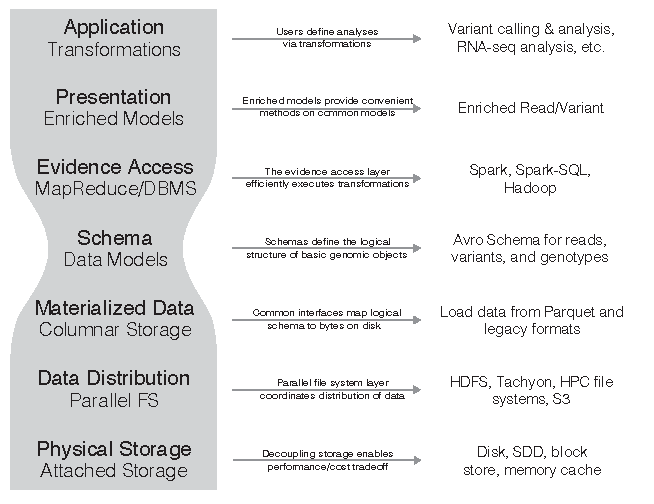
\includegraphics[width=0.75\linewidth]{expanded-stack-2.pdf}
\end{center}
\caption{A Stack Model for Genomic Analyses}
\label{fig:stack-model}
\end{figure}

While the abstraction inversion used in genomics to accelerate common access patterns is undesirable
because it violates data independence, we also find that it sacrifices performance and
accuracy. The current Sequence/Binary Alignment and Map~(SAM/BAM~\cite{li09}) formats for storing
genomic alignments apply constraints about record ordering to enable specific computing patterns. Our
implementation~(described in~\S\ref{sec:genomics-pipeline}) identifies errors in two current genomics
processing stages that occur \emph{because} of the sorted access invariant. Our implementations of
these stages do not make use of sort order, and achieve higher performance \emph{while} eliminating
these errors.

Additionally, this thesis describes the variant discovery and genotyping algorithms implemented in
\texttt{avocado}. \texttt{avocado} introduces a new algorithm for local reassembly that eliminates the
expensive step of realigning reads to candidate haplotypes. Additionally, \texttt{avocado} introduces
a novel statistical model for genotyping that eliminates errors caused by statistical models that
optimistically assume the local independence of genomic loci.

All of the software~(source code and executables) described in this thesis are available free of charge
under the permissive Apache 2 open-source license. \texttt{ADAM} is available at
\url{https://www.github.com/bigdatagenomics/adam}, and \texttt{avocado} is available at
\url{https://www.github.com/bigdatagenomics/avocado}.

\section{Background}
\label{sec:background}

This work is at the intersection of computational biology, data management, and processing
systems. As such, our architectural approach is informed by recent trends in both areas. The design of
large scale data management systems has changed dramatically since the papers by Dean and
Ghemawat~\cite{dean04, dean08} describing Google's \texttt{MapReduce} system. Over a
similar timeframe, genomics has arisen due to improvements in data acquisition technologies. For
example, since the Human Genome Project finished in 2001~\cite{lander01}, the price of genomic
sequencing has dropped by 10,000$\times$~\cite{nhgri}. This drop in cost has enabled the capture of
petabytes of sequence data, which has (in turn) enabled significant population genomics experiments like 
the 1000 Genomes project~\cite{siva08} and The Cancer Genome Atlas~(TCGA, \cite{weinstein13}).

Although there has been significant progress in the development of systems for processing large
datasets---the development of first generation MapReduce systems~\cite{dean04}, followed by
iterative MapReduce systems like Spark~\cite{zaharia10}, as well as parallel and columnar
DBMS~\cite{abadi06, lamb12}---the uptake of these systems in genomics has been slow.
\texttt{MapReduce}'s impact has been limited to tools that use the map-reduce programming model as an
inspiration for API design~\cite{mckenna10}, or have been limited systems that have used \texttt{Hadoop}
to na\"{i}vely parallelize existing toolkits~\cite{langmead09, schatz09}. These approaches are perilous for
several reasons:

\begin{itemize}
\item A strong criticism levied against the MapReduce model is that the API is insufficiently expressive
for describing complex tasks. As a consequence of this, tools like the GATK~\cite{mckenna10} that
adopt MapReduce as a programming model force significant restrictions on algorithm implementors. For
example, a GATK \texttt{walker}\footnote{The GATK provides \texttt{walker}s as an interface for
traversing regions of the genome.} is provided with a single view over the data~(a sorted iterator over a
specified region), and is allowed limited reduce functionality.
\item A major contribution of systems like MapReduce~\cite{dean08} and Spark~\cite{zaharia10,
zaharia12} is the ability to reliably distribute parallel tasks across a cluster in an automated fashion. While
the GATK uses MapReduce as a programming abstraction~(i.e., as an interface for writing
\texttt{walker}s), it does not use MapReduce as an execution strategy. To run tools like the GATK across
a cluster, organizations use workflow management systems for sharding and persisting intermediate
data, and managing failures and retries. This approach is not only an inefficient duplication of work, but it
is also a source of inefficiency during execution: the performance of iterative stages in the GATK is
bottlenecked by I/O performance.
\item The na\"{i}ve Hadoop-based implementations in Crossbow~\cite{langmead09} and
Cloudburst~\cite{schatz09} use scripts to run unmodified legacy tools on top of Hadoop. This approach
does achieve speedups, but does not attack overhead. Several of the methods that they parallelize
incur high overhead due to duplicated loading of indices (for fast aligners, loading of large indices can be
a primary I/O bottleneck) and poor broadcasting of data.
\end{itemize}

Recent work by Diao et al~\cite{diao15} has looked at optimizations to MapReduce systems for
processing genomic data. They adapt strategies from the query optimization literature to reorder
computation to minimize data shuffling. While this approach does improve shuffle traffic, several
preprocessing stages cannot be transposed. For instance, reversing the order of indel realignment and
base quality score recalibration~(see~\S\ref{sec:genomics-pipeline}) will change the inferred quality
score distribution. Additionally, we believe that the shuffle traffic that Diao et al observe is an artifact
caused by an abstraction inversion present in many genomics tools. This abstraction inversion requires
that all genomic data is processed in sorted order, which necessitates frequent shuffles. As we
demonstrate in~\S\ref{sec:genomics-pipeline}, these penalties can be eliminated by restructuring the
pre-processing algorithms.

One notable area where modern data management techniques have been leveraged by scientists is in
the data storage layer. Due to the storage costs of large genomic datasets, scientists have introduced the
CRAM format that uses columnar storage techniques and special compression algorithms to achieve a
30\% reduction in size over the original BAM format~\cite{fritz11}. While CRAM achieves high~($\gg
50\%$) compression, it imposes restrictions on the ordering and structure of the data, and does not
provide support for predicates or projection. We perform a more comprehensive comparison against
CRAM in~\S\ref{sec:column-store-perf}.

One interesting trend of note is the development of databases specifically for scientific applications.
The exemplar is SciDB, which provides an array based storage model as well as efficient
linear algebra routines~\cite{brown10}. While arrays accelerate many linear algebra based routines, they
are not a universally great fit. For many genomics workloads, data is semistructured and may consist of
strings, boolean fields, and an array of tagged annotations. Other systems like the Genome Query
Language~\cite{kozanitis14} have extended SQL to provide efficient query semantics across genomic
coordinates. While GQL achieves performance improvements of up to 10$\times$ for certain algorithms,
SQL is not an attractive language for many scientific domains, which make heavy use of user designed
functions that may be cumbersome in SQL.

\section{Pipeline Structure}
\label{sec:genomics-pipeline}

This thesis targets the acceleration of \emph{variant calling}, which is a statistical process to infer the
sites at that a single individual varies from the reference genome.\footnote{The reference genome
represents the ``average'' genome for a species. The Human Genome Project~\cite{lander01} assembled
the first human reference genome.} Although there are a variety of sequencing technologies in use, the
majority of sequence data used for variant calling and genotyping comes from the Illumina sequencing
platform, which uses a ``sequencing-by-synthesis'' technique to generate short read
data~\cite{metzker09}. Short read refers to 
sequencing run will generate many reads that are between 50 and 250 bases in length. In addition to
adjusting the length of the reads, we can control the amount of the data that is generated by
changing the amount of the genome that we sequence, or the amount of redundant sequencing that
we perform~(the average number of reads that covers each base, or \emph{coverage}). A single
human genome sequenced at 60$\times$ coverage will produce approximately 1.4 billion reads,
which is approximately 600 GB of raw data, or 225 GB of compressed data. For each read, we also
are provided \emph{quality scores}, which represent the likelihood that the base at a given position
was observed. In a variant calling pipeline, we perform the following steps:

\begin{enumerate}
\item \textbf{Alignment:} For each read, we find the position in the genome that the read is most likely to
have come from. As an exact search is too expensive, there has been an extensive amount of research
that has focused on indexing strategies for improving alignment performance~\cite{li10, li11wham,
zaharia11}. This process is parallel per sequenced read.
\item \textbf{Pre-processing:} After reads have been aligned to the genome, we perform several
preprocessing steps to eliminate systemic errors in the reads. This may involve recalibrating the
observed quality scores for the bases, or locally optimizing the read alignments. We will present a
description of several of these algorithms in~\S\ref{sec:genomics-pipeline}; for a more detailed
discussion, we refer readers to DePristo et al~\cite{depristo11}.
\item \textbf{Variant calling:} Variant calling is a statistical process that uses the read alignments
and the observed quality scores to compute whether a given sample matches or diverges
from the reference genome. This process is typically parallel per position or region in the genome.
\item \textbf{Filtration:} After variants have been called, we want to filter out false positive variant calls.
We may perform queries to look for variants with borderline likelihoods, or we may look for clusters of
variants, which may indicate that a local error has occurred. This process may be parallel per position,
may involve complex traversals of the genomic coordinate space, or may require us to fit a statistical
model to all or part of the dataset.
\end{enumerate}

This process is very expensive in time to run; the current best practice pipeline uses the BWA
tool~\cite{li10} for alignment and the GATK~\cite{depristo11, mckenna10} for pre-processing, variant
calling, and filtration. Current benchmark suites have measured this pipeline as taking between 90 and
130 hours to run end-to-end~\cite{talwalkar14}. Recent projects have achieved 5--$10\times$
improvements in alignment and variant calling performance~\cite{rimmer14, zaharia11}, which makes the
pre-processing stages the performance bottleneck. Our experimental results have corroborated this, as
the four pre-processing stages take over 110 hours to run on a clinical quality human genome when run
on an Amazon EC2 \texttt{cr1.8xlarge} machine. 

For current implementations of these read processing steps, performance is limited by disk
bandwidth~\cite{diao15}. This bottleneck exists because the operations read in a SAM/BAM file, perform
a small amount of processing, and write the data to disk as a new SAM/BAM file. We achieve a
performance bump by performing our processing iteratively in memory. The four read processing stages
can then be chained together, eliminating three long writes to disk and an additional three long reads
from disk. Additionally, by rethinking the design of our algorithms, we are able to reduce overhead in
several other ways:

\begin{enumerate}
\item Current algorithms require the reference genome to be present on all nodes. This assembly is then
used to look up the reference sequence that overlaps all reads. The reference genome is several
gigabytes in size, and performing a lookup in the reference genome can be costly due to its size. Instead,
wherever possible, we leverage the \texttt{mismatchingPositions} field in our schema to embed
information about the reference in each read. This optimization allows us to avoid broadcasting the
reference, and provides O(1) lookup. When this is not possible, we make use of a ``region join'' primitive,
which enables us to make use of the reference genome with \emph{minimal} duplication.
\item Shared-memory genomics applications tend to be impacted significantly by false sharing of data
structures~\cite{zaharia11}. Instead of having data structures that are modified in parallel, we
restructure our algorithms so that we only touch data structures from a single thread, and then merge
structures in a reduce phase. The elimination of sharing improves the performance of covariate
calculation during BQSR and the target generation phase of local realignment.
\item In a na\"{i}ve implementation, the local realignment and duplicate marking tasks can suffer from
stragglers. The stragglers occur due to a large amount of reads that either do not associate to a
realignment target, or that are unaligned. We pay special attention to these cases by manually
randomizing the partitioning for these reads. This resolves load imbalance and mitigates stragglers.
\item For the Flagstat command, we are able to project a limited subset of fields. Flagstat touches fewer
than 10 fields, which account for less than 10\% of space on disk. We discuss the performance
implications of this further in~\S\ref{sec:column-store-perf}.
\end{enumerate}

These techniques allow us to achieve a $>50\times$ performance improvement over current tools, and
scalability beyond 128 machines. We perform a detailed performance review
in~\S\ref{sec:genomics-performance}.

\section{Related Work}
\label{sec:related-work}

Several variant analysis toolkits exist, with the most well known analysis toolkit being the
\texttt{GATK}~\cite{depristo11}. Additional toolkits include \texttt{HugeSeq}~\cite{lam12},
\texttt{STORMSeq}~\cite{karczewski14}, and \texttt{SpeedSeq}~\cite{chiang14}. These tools combine
alignment, variant calling, and filtration into an easy to use package, and may also orchestrate
work distribution across a set of distributed machines. For example, the \texttt{GATK} and
\texttt{HugeSeq} make use of an improvised map-reduce model, while \texttt{STORMSeq} uses a grid
engine to distribute work according to a provided partitioning function. These tools delegate to either
the \texttt{GATK}'s \texttt{HaplotypeCaller} or \texttt{UnifiedGenotyper}, or
\texttt{FreeBayes}~\cite{garrison12} for calling germline point events and INDELs.
\texttt{Platypus}~\cite{rimmer14} is an additional notable toolkit that directly integrates alignment with
variant calling to improve computational efficiency.

Although earlier methods such as the \texttt{mpileup} caller assumed the statistical independence of
sites~\cite{li11snp} post-alignment, current variant calling pipelines depend heavily on realignment based
approaches for accurate genotyping~\cite{li14}. These methods take two different approaches to generate candidate sequences for realignment:

\begin{enumerate}
\item \emph{Realignment-only:} Putative INDELs are extracted directly from the aligned reads, and the
reads are locally realigned,
\item \emph{Reassembly:} The aligned reads are reassembled into haplotypes, which the reads are
aligned against.
\end{enumerate}

The realignment-only approach is used in \texttt{UnifiedGenotyper}\footnote{When used following
\texttt{IndelRealignment}} and \texttt{FreeBayes}, while \texttt{HaplotypeCaller}, \texttt{Platypus}, and
\texttt{Scalpel}~\cite{narzisi14} make use of reassembly. In both cases, we perform the following
algorithmic steps:

\begin{enumerate}
\item Candidate haplotypes are generated for realignment,
\item Each read is realigned to each haplotype, typically using a pair Hidden Markov Model~(HMM,
see~\cite{durbin98}),
\item A statistical model uses the read$\leftrightarrow$haplotype alignments to choose the haplotype pair
that most likely represents the variants hypothesized to exist in the region, 
\item The alignments of the reads to the chosen haplotype pair are used to generate statistics that are
then used for genotyping.
\end{enumerate}

In haplotype reassembly, step 1 is broken down into two further steps:

\begin{enumerate}
\item A \emph{de Bruijn} graph is constructed from the reads aligned to a region of the reference genome,
\item All valid paths between the start and end of the graph are enumerated.
\end{enumerate}

In both the \emph{realignment} and \emph{reassembly} approaches, local alignment errors~(errors in
alignment \emph{within} this region) are corrected by using a statistical model to identify the most likely
location that the read could have come from, given the other reads seen in this area. These approaches
are algorithmically different from \emph{global alignment} because they make use of local context when
picking the sequence to align to, and the alignment search space is much smaller, which enables the use
of more expensive alignment methods.

\emph{De novo} assembly provides another promising approach to variant discovery. In the \emph{de
novo} formulation of assembly, the reads are not aligned to a reference genome. Instead, ``novel''
contiguous fragments of sequence are assembled from the reads. Variants are called by aligning these
assemblies to the reference genome, and by realigning the reads against the novel assemblies. Several
implementations of \emph{de novo} variant calling exist, most notably the \texttt{Cortex}~\cite{iqbal12}
and \texttt{Discovar}~\cite{weisenfeld14} assemblers. Although \emph{de novo} assembly solves
several important issues seen by traditional variant callers~(reference bias, structural variant detection),
\emph{de novo} assembly is currently too computationally expensive for widespread use in genotyping.

\chapter{Genomic Data Storage and Preprocessing Using \texttt{ADAM}}

\section{Distributed Architectures for Genomics}
\label{sec:distributed-architectures}

Due to both the growing volume of genomic sequencing data and the large size of these datasets,
sequencing centers face the increasingly difficult task of turning around genomic data analyses in a
reasonable timeframe~\cite{schadt10, stein10}. While the per-run latency of current genomic pipelines
such as the \texttt{GATK} can be improved by manually partitioning the input dataset and distributing
work, native support for distributed computing is not provided. As a stopgap solution, projects like
\texttt{Cloudburst}~\cite{schatz09} and \texttt{Crossbow}~\cite{langmead09} have ported individual
analytics tools to run on top of Hadoop. While this approach has served well for proofs of concept,
it provides poor abstractions for application developers and makes it difficult to create novel distributed
genomic analyses, and does little to attack sources of inefficiency or incorrectness in distributed
genomics pipelines.

To address these problems, we need to reconsider how to build software for processing genomic data.
Modern genome analysis pipelines are built around monolithic architectures and flat file formats.
These architectures are designed to efficiently run current algorithms on single node processing
systems, but impose significant restrictions. These restrictions include:

\begin{itemize}
\item These implementations are locked to a single node processing model. Even the \texttt{GATK}'s
``map-reduce'' styled \texttt{walker} API~\cite{mckenna10} is limited to natively support processing on
a single node. While these jobs can be manually partitioned and run in a distributed setting, manual
partitioning can lead to imbalance in work distribution and makes it difficult to run algorithms that
require aggregating data across all partitions, and lacks the fault tolerance provided by modern
distributed systems such as Hadoop or Spark~\cite{zaharia12}.
\item Most of these implementations \emph{assume} invariants about the sorted order of records on
disk. This ``stack smashing'' (specifically, the layout of data is used to ``accelerate'' a processing stage)
can lead to bugs when data does not cleanly map to the assumed sort order. Additionally, since these
sort order invariants are rarely explicit and vary from tool to tool, pipelines assembled from disparate
tools can be brittle.
\item Additionally, while these invariants are intended to improve performance, it is not clear that these
invariants \emph{actually} improve performance. There are two common sort invariants used in genomics:
sort by reference position, and sort by read name. Changing between these two sort orders entails
a full shuffle and resort of the dataset. Additionally, a sort is required after alignment to establish a sort order.
\end{itemize}

As noted above, current implementations are locked to a single node model. Projects like
\texttt{Hadoop-BAM}~\cite{niemenmaa12}, \texttt{SeqPig}~\cite{schumacher14}, and \texttt{BioPig}~\cite{nordberg13}
have attempted to build a distributed processing environment on top of current single node genomics APIs.
However, several problems must be solved in order to make distributed processing of genomic data productive:

\begin{itemize}
\item Current genomics data formats rely on a centralized header for storing experiment metadata. Since the
metadata is centralized, it must be replicated to all machines.
\item A simple map-reduce or SQL-like API is insufficient for implementing genomic analyses. Rather, to enhance
bioinformatician productivity, we need to define APIs that allow developers to conveniently express algorithms.
\end{itemize}

In \texttt{ADAM}, we have taken a more aggressive approach to the design of APIs for processing genomic data
in a distributed system. Although modern genomics pipelines are built as monolithic applications, we have
chosen a layered decomposition for \texttt{ADAM}, that uses a schema as a ``narrow waist''. Instead of using
a flat file format, as is traditional in genomics, we are using this schema with Parquet~(a commodity columnar
store,~\cite{parquet}) to store genomic data in a way that both allows efficient distributed read/write and that
achieves high compression. On top of this, we have added primitives that implement common genomic traversals
in a distributed manner. We have then used \texttt{ADAM} to implement common preprocessing stages from
commonly used genomics pipelines. \texttt{ADAM}'s preprocessing stages are between 1-5$\times$ faster than the
equivalent \texttt{GATK} preprocessing stages, and achieve linear scaling out to 128 nodes.

\section{Layering}
\label{sec:layering}

The processing patterns being applied to scientific data shift widely as the data itself ages. Because of
this change, we want to design a scientific data processing system that is flexible enough to
accommodate our different use cases. At the same time, we want to ensure that the components in the
system are well isolated so that we avoid bleeding functionality across the stack. If we bleed functionality
across layers in the stack, we make it more difficult to adapt our stack to different applications.
Additionally, as we discuss in~\S\ref{sec:genomics-pipeline}, improper separation of concerns can
actually lead to errors in our application.

These concerns are very similar to the factors that led to the development of the Open Systems
Interconnection~(OSI) model and Internet Protocol~(IP) stack for networking
services~\cite{zimmermann80}. The networking stack models were designed to allow the mixing and
matching of different protocols, all of which existed at different functional levels. The success of the
networking stack model can largely be attributed to the ``narrow waist'' of the stack, which simplified the
integration of a new protocol or technology by ensuring that the protocol only needed to implement a
single interface to be compatible with the rest of the stack.

Unlike conventional scientific systems that leverage custom data formats like BAM/SAM~\cite{li09},
or CRAM~\cite{fritz11}, we believe that the use of an explicit schema for data interchange is critical.
In our stack model shown in Figure~\ref{fig:stack-model}, the schema becomes the ``narrow waist''
of the stack. Most importantly, placing the schema as the narrow waist enforces a strict separation
between data storage/access and data processing. Additionally, this enables literate programming
techniques which can clarify the data model and access patterns. The seven layers of our stack model
are decomposed as follows, and are numbered in ascending order from bottom to top:

\begin{enumerate}
\item \textbf{Physical Storage:} This layer coordinates data writes to physical media.
\item \textbf{Data Distribution:} This layer manages access, replication, and distribution of the files that have
been written to storage media.
\item \textbf{Materialized Data:} This layer encodes the patterns for how data is encoded and stored. This
layer determines I/O bandwidth and compression.
\item \textbf{Data Schema:} This layer specifies the representation of data, and forms the narrow waist of
the stack that separates access from execution.
\item \textbf{Evidence Access:} This layer provides us with primitives for processing data, and allows us to
transform data into different views and traversals.
\item \textbf{Presentation:} This layer enhances the data schema with convenience methods for performing
common tasks and accessing common derived fields from a single element.
\item \textbf{Application:} At this level, we can use our evidence access and presentation layers to compose
the algorithms to perform our desired analysis.
\end{enumerate}

A well defined software stack has several other significant advantages. By limiting application
interactions with layers lower than the presentation layer, application developers are given a clear and
consistent view of the data they are processing, and this view of the data is independent of whether the
data is local or distributed across a cluster or cloud. By separating the API from the data access layer,
we improve flexibility. With careful design in the data format and data access layers, we can seamlessly
support conventional whole file access patterns, while also allowing easy access to small slices of files.
By treating the compute substrate and storage as separate layers, we also drastically increase
the portability of the APIs that we implement.

As we discuss in more detail in~\S\ref{sec:genomics-pipeline}, current scientific systems bleed
functionality between stack layers. An exemplar is the SAM/BAM and CRAM formats, which expect data
to be sorted by genomic coordinate. This modifies the layout of data on disk~(level 3, Materialized Data)
and constrains how applications traverse datasets~(level 5, Evidence Access). Beyond
constraining applications, this leads to bugs in applications that are difficult to detect.\footnote{The
current best-practice implementations of the BQSR and Duplicate Marking algorithms both fail when
processing certain corner-case alignments. These errors are caused because of the requirement to
traversing reads in sorted order.} These views of evidence should be implemented at the evidence
access layer instead of in the layout of data on disk. This enforces independence of anything below the
schema.

The idea of decomposing scientific applications into a stack model is not new; Bafna et al~\cite{bafna13}
made a similar suggestion in 2013. We borrow some vocabulary from Bafna et al, but our approach is
differentiated in several critical ways:

\begin{itemize}
\item Bafna et al consider the stack model specifically in the context of data management systems for
genomics; as a result, they bake current technologies and design patterns into the stack. In our opinion,
a stack design should serve to abstract layers from methodologies/implementations. If not, future
technology trends may obsolete a layer of the stack and render the stack irrelevant.
\item Bafna et al define a binary data format as the narrow waist in their stack, instead of a schema.
While these two seem interchangeable, they are not in practice. A schema is a higher level of abstraction
that encourages the use of literate programming techniques and allows for data serialization techniques
to be changed as long as the same schema is still provided.
\item Notably, Bafna et al use this stack model to motivate GQL~\cite{kozanitis14}. While a query system
should provide a way to process and transform data, Bafna et al instead move this system down to the
data materialization layer. We feel that this inverts the semantics that a user of the system would prefer
and makes the system less general.
\end{itemize}

Deep stacks like the OSI stack~\cite{zimmermann80} are generally simplified for practical use. Conceptually,
the stack we propose is no exception. In practice, we combine layers one and two, and layers five and six.
There are several reasons for this. First, in Hadoop-based systems, the system does not have practical visibility
below layer two, thus there is no reason to split layers one and two except as a philosophical exercise.
Layers five and six are commingled because some of the enriched presentation objects are used to
implement functionality in the evidence access layer. This normally happens when a key is needed, such as
when repartitioning the dataset, or when reducing or grouping values.

\section{Data Storage for Genomic Data}
\label{sec:schema-design}

A common criticism of bioinformatics as a field surrounds the proliferation of file formats. Short read data alone is
stored in four common formats: \texttt{FASTQ}~\cite{cock10}, \texttt{SAM}/\texttt{BAM}~\cite{li09}, and
\texttt{CRAM}~\cite{fritz11}. While these formats all represent different layouts of data on disk, they tend to be
logically harmonious. Due to this logical congruency of the different formats, we chose to build \texttt{ADAM}
on top of a logical schema, instead of a binary format on disk. While we do use Apache \texttt{Parquet}~\cite{parquet} to
materialize data on disk, the Apache \texttt{Avro}~\cite{avro} schema is used as a narrow waist in the system,
that enables ``legacy'' formats to be processed identically to data stored in \texttt{Parquet}.

We made several high level choices when designing the schemas used in \texttt{ADAM}. First, the schemas are fully
denormalized, which reduces the cost of metadata access and simplifies metadata distribution. We are able to
get these benefits without greatly increasing the cost of memory access because our backing store~(\texttt{Parquet})
makes use of run length and dictionary encoding, which allows for a single object to be allocated for highly repetitive
elements on read. Another key design choice was to require that all fields in the schema are nullable; by enforcing
this requirement, we enable arbitrary user specified projections. Arbitrary projections can be used to accelerate
common sequence quality control algorithms such as Flagstat~\cite{massie13, nothaft15}.

We have reproduced the schemas used to describe reads, variants, and genotypes below. \texttt{ADAM} also
contains schemas for describing assembled contigs, genomic features, and variant annotations, but we have
not included them in this section.

\begin{lstlisting}[caption=\texttt{ADAM} read schema]
record AlignmentRecord {
  /** Alignment position and quality */
  Contig contig;
  long start;
  long oldPosition;
  long end;

  /** read ID, sequence, and quality */
  string readName;
  string sequence;
  string qual;
  
  /** alignment details */
  string cigar;
  string oldCigar;
  int mapq;
  int basesTrimmedFromStart;
  int basesTrimmedFromEnd;
  boolean readNegativeStrand;
  boolean mateNegativeStrand;
  boolean primaryAlignment;
  boolean secondaryAlignment;
  boolean supplementaryAlignment;
  string mismatchingPositions;
  string origQual;

  /** Read status flags */
  boolean readPaired;
  boolean properPair;
  boolean readMapped;
  boolean mateMapped;
  boolean firstOfPair;
  boolean secondOfPair;
  boolean failedVendorQualityChecks;
  boolean duplicateRead;

  /** optional attributes */
  string attributes;

  /** record group metadata */
  string recordGroupName;
  string recordGroupSequencingCenter;
  string recordGroupDescription;
  long recordGroupRunDateEpoch;
  string recordGroupFlowOrder;
  string recordGroupKeySequence;
  string recordGroupLibrary;
  int recordGroupPredictedMedianInsertSize;
  string recordGroupPlatform;
  string recordGroupPlatformUnit;
  string recordGroupSample;

  /** Mate pair alignment information */
  long mateAlignmentStart;
  long mateAlignmentEnd;
  Contig mateContig;
}
\end{lstlisting}

Our read schema maps closely to the logical layout of data presented by \texttt{SAM} and \texttt{BAM}.
The main modifications relate to how we represent metadata, which has been denormalized across the record.
All of the metadata from the sequencing run and prior processing steps are packed into the record
group metadata fields. The program information describes the processing lineage of the sample and
is expected to be uniform across all records, thus it compresses extremely well. The record group
information is not guaranteed to be uniform across all records, but there are a limited number number
of record groups per sequencing dataset. This
metadata is string heavy, which makes proper deserialization from disk important. Although the
information consumes less than 5\% of space on disk, a poor deserializer implementation may replicate
a string per field per record, which greatly increases the amount of memory allocated and the garbage
collection~(GC) load.

\begin{lstlisting}[caption=\texttt{ADAM} variant and genotype schemas]
enum StructuralVariantType {
  DELETION,
  INSERTION,
  INVERSION,
  MOBILE_INSERTION,
  MOBILE_DELETION,
  DUPLICATION,
  TANDEM_DUPLICATION
}

record StructuralVariant {
  StructuralVariantType type;
  string assembly;

  boolean precise;
  int startWindow;
  int endWindow;
}

record Variant {
  Contig contig;
  long start;
  long end;

  string referenceAllele;
  string alternateAllele;
  StructuralVariant svAllele;

  boolean isSomatic;
}

enum GenotypeAllele {
  Ref,
  Alt,
  OtherAlt,
  NoCall
}

record VariantCallingAnnotations {
  float variantCallErrorProbability;

  array<string> variantFilters;

  int readDepth;
  boolean downsampled;
  float baseQRankSum;
  float clippingRankSum;
  float fisherStrandBiasPValue = null;
  float haplotypeScore;
  float inbreedingCoefficient;
  float rmsMapQ;
  int mapq0Reads;
  float mqRankSum;
  float variantQualityByDepth;
  float readPositionRankSum;

  array<int> genotypePriors;
  array<int> genotypePosteriors;

  float vqslod;
  string culprit;
  boolean usedForNegativeTrainingSet;
  boolean usedForPositiveTrainingSet;

  map<string> attributes;
}

record Genotype {
  Variant variant;
  VariantCallingAnnotations variantCallingAnnotations;

  string sampleId;
  string sampleDescription;
  string processingDescription;

  array<GenotypeAllele> alleles;

  float expectedAlleleDosage;
  int referenceReadDepth;
  int alternateReadDepth;
  int readDepth;
  int minReadDepth;
  int genotypeQuality;
  array<int> genotypeLikelihoods;
  array<int> nonReferenceLikelihoods;
  array<int> strandBiasComponents;

  boolean splitFromMultiAllelic;

  boolean isPhased;
  int phaseSetId;
  int phaseQuality;
}
\end{lstlisting}

The variant and genotype schemas present a larger departure from the representation used by the Variant Call
Format~(\texttt{VCF}). The most noticeable difference is that we have migrated away from \texttt{VCF}'s variant oriented
representation, to a matrix representation. Instead of the variant record serving to group together genotypes, the
variant record is embedded within the genotype. Thus, a record represents the genotype assigned to a sample,
as opposed to a \texttt{VCF} row, where all individuals are collected together. The second major modification that we
make is to assume a biallelic representation. This differs from \texttt{VCF}, which allows multiallelic records. By limiting
ourselves to a biallelic representation, we are able to clarify the meaning of many of the variant calling annotations. If a
site contains a multiallelic variant (e.g., in \texttt{VCF} parlance this could be a \texttt{1/2} genotype), we split the
variant into two or more biallelic records. The sufficient statistics for each allele should then be computed under
a reference model similar to the model used in genome \texttt{VCF}s. If the sample does contain a multiallelic variant at
the given site, this multiallelic variant is represented by referencing to another record via the \texttt{OtherAlt}
enumeration.

These representations achieve high compression versus the legacy formats. We provide a detailed breakdown of
compression in more in~\S\ref{sec:compression}. \texttt{ADAM} data stored in \texttt{Parquet} achieves an
approximately 25\% improvement in file size over compressed \texttt{BAM} for read data, and a 66\% improvement
over \texttt{GZIP}ped \texttt{VCF} for variant data.

\section{Read Preprocessing Algorithms}
\label{sec:read-preprocessing}

In \texttt{ADAM}, we have implemented the three most-commonly used pre-processing stages from the
\texttt{GATK} pipeline~\cite{depristo11}. In this section, we describe the stages that we have
implemented, and the techniques we have used to improve performance and accuracy when running on
a distributed system. These pre-processing stages include:

\begin{enumerate}
\item \textbf{Duplicate Removal:} During the process of preparing DNA for sequencing, reads are duplicated by
errors during the sample preparation and polymerase chain reaction stages. Detection of duplicate reads
requires matching all reads by their position and orientation after read alignment. Reads with identical position
and orientation are assumed to be duplicates. When a group of duplicate reads is found, each read is scored,
and all but the highest quality read are marked as duplicates.

We have validated our duplicate removal code against Picard~\cite{picard}, which is used by the GATK
for Marking Duplicates. Our implementation is fully concordant with the Picard/GATK duplicate removal
engine, except we are able to perform duplicate marking for chimeric read pairs.\footnote{In a chimeric read pair,
the two reads in the read pairs align to different chromosomes; see Li et al~\cite{li10}.}
Specifically, because Picard's traversal engine is restricted to processing linearly sorted alignments,
Picard mishandles these alignments. Since our engine is not constrained by the underlying layout of data
on disk, we are able to properly handle chimeric read pairs.
\item \textbf{Local Realignment:} In local realignment, we correct areas where variant alleles cause reads to be
locally misaligned from the reference genome.\footnote{This is typically caused by the presence of
insertion/deletion (INDEL) variants; see DePristo et al~\cite{depristo11}.} In this algorithm, we first identify regions
as targets for realignment. In the GATK, this is done by traversing sorted read alignments. In our implementation,
we fold over partitions where we generate targets, and then we merge the tree of targets. This process allows us
to eliminate the data shuffle needed to achieve the sorted ordering. As part of this fold, we must
compute the convex hull of overlapping regions in parallel. We discuss this in more detail in
Appendix~\ref{sec:convex-hull}.

After we have generated the targets, we associate reads to the overlapping target, if one exists. After
associating reads to realignment targets, we run a heuristic realignment algorithm that works by minimizing
the quality-score weighted number of bases that mismatch against the reference.
\item \textbf{Base Quality Score Recalibration~(BQSR):} During the sequencing process, systemic errors occur
that lead to the incorrect assignment of base quality scores. In this step, we label each base that we have
sequenced with an \emph{error covariate}. For each covariate, we count the total number of bases that we saw,
as well as the total number of bases within the covariate that do not match the reference genome. From this data, 
we apply a correction by estimating the error probability for each set of covariates under a beta-binomial model
with uniform prior.

We have validated the concordance of our BQSR implementation against the GATK. Across both tools, only 5000
of the $\sim$180B bases~($<0.0001\%$) in the high-coverage NA12878 genome dataset differ. After investigating
this discrepancy, we have determined that this is due to an error in the GATK, where paired-end reads are
mishandled if the two reads in the pair overlap.
\end{enumerate}

In the rest of this section, we discuss the high level implementations of these algorithms.

\subsection{BQSR Implementation}
\label{sec:bqsr-implementation}

Base quality score recalibration seeks to identify and correct correlated errors in base quality score estimates.
At a high level, this is done by associating sequenced bases with possible error covariates, and estimating the
true error rate of this covariate. Once the true error rate of all covariates has been estimated, we then apply
the corrected covariate.

Our system is generic and places no limitation on the number or type of covariates that can be applied. A covariate
describes a parameter space where variation in the covariate parameter may be correlated with a sequencing
error. We provide two common covariates that map to common sequencing errors~\cite{nakamura11}:

\begin{itemize}
\item \emph{CycleCovariate}: This covariate expresses which cycle the base was sequenced in. Read errors are
known to occur most frequently at the start or end of reads.
\item \emph{DinucCovariate}: This covariate covers biases due to the sequence context surrounding a site. The 2-mer
ending at the sequenced base is used as the covariate parameter value.
\end{itemize}

To generate the covariate observation table, we aggregate together the number of observed and error bases per
covariate. This process is demonstrated in Algorithms~\ref{alg:emit-observations} and \ref{alg:create-table}.

\begin{algorithm}
\caption{Emit Observed Covariates}
\label{alg:emit-observations}
\begin{algorithmic}
\STATE $read \leftarrow$ the read to observe
\STATE $covariates \leftarrow$ covariates to use for recalibration
\STATE $sites \leftarrow$ sites of known variation
\STATE $observations \leftarrow \emptyset$
\FOR{$base \in read$}
\STATE $covariate \leftarrow$ identifyCovariate($base$)
\IF{isUnknownSNP($base, sites$)}
\STATE $observation \leftarrow$ Observation($1, 1$)
\ELSE
\STATE $observation \leftarrow$ Observation($1, 0$)
\ENDIF
\STATE $observations$.append($(covariate, observation)$)
\ENDFOR
\RETURN $observations$
\end{algorithmic}
\end{algorithm}

\begin{algorithm}
\caption{Create Covariate Table}
\label{alg:create-table}
\begin{algorithmic}
\STATE $reads \leftarrow$ input dataset
\STATE $covariates \leftarrow$ covariates to use for recalibration
\STATE $sites \leftarrow$ known variant sites
\STATE $sites$.broadcast()
\STATE $observations \leftarrow reads$.map($read \rightarrow$ emitObservations($read, covariates, sites$))
\STATE $table \leftarrow$ $observations$.aggregate(CovariateTable(), mergeCovariates)
\RETURN $table$
\end{algorithmic}
\end{algorithm}

In Algorithm~\ref{alg:emit-observations}, the \texttt{Observation} class stores the number of bases seen
and the number of errors seen. For example, \texttt{Observation(1, 1)} creates an \texttt{Observation} object
that has seen one base, which was an erroneous base.

Once we have computed the observations that correspond to each covariate, we estimate the observed base
quality using equation~\eqref{eqn:bqsr-err}. This represents a Bayesian model of the mismatch probability with
Binomial likelihood and a Beta(1, 1) prior.

\begin{equation}
\label{eqn:bqsr-err}
\mathbf{E}(P_{err}|{cov}) = \frac{\texttt{\#errors}(cov) + 1}{\texttt{\#observations}(cov) + 2}
\end{equation}

After these probabilities are estimated, we go back across the input read dataset and reconstruct the quality
scores of the read by using the covariate assigned to the read to look into the covariate table.

\subsection{Indel Realignment Implementation}
\label{sec:indel-realignment-implementation}

Although global alignment will frequently succeed at aligning reads to the proper region of the genome, the local
alignment of the read may be incorrect. Specifically, the error models used by aligners may penalize local alignments
containing INDELs more than a local alignment that converts the alignment to a series of mismatches. To correct
for this, we perform local realignment of the reads against consensus sequences. This is implemented as a three step
process. In the first step, we identify candidate sites that have evidence of an insertion or deletion. We then compute
the convex hull of these candidate sites, to determine the windows we need to realign over. After these regions are
identified, we generate candidate haplotype sequences, and realign reads to minimize the overall quantity of mismatches
in the region.

\subsubsection{Realignment Target Identification}
\label{sec:realignment-target-identification}

To identify target regions for realignment, we simply map across all the reads. If a read contains INDEL evidence,
we then emit a region corresponding to the region covered by that read.

\subsubsection{Convex-Hull Finding}
\label{sec:convex-hull}

Once we have identified the target realignment regions, we must then find the maximal convex hulls
across the set of regions. For a set $R$ of regions, we define a maximal convex hull as the largest
region $\hat{r}$ that satisfies the following properties:

\begin{align}
\label{eqn:convexity-constraint}
\hat{r} &= \cup_{r_i \in \hat{R}} r_i \\
\hat{r} \cap r_i &\ne \emptyset, \forall r_i \in \hat{R} \\
\hat{R} &\subset R
\end{align}

In our problem, we seek to find all of the maximal convex hulls, given a set of regions. For genomics, the
convexity constraint described by equation \eqref{eqn:convexity-constraint} is trivial to check: specifically, the
genome is assembled out of reference contigs\footnote{\emph{Contig} is short for \emph{contiguous
sequence}. In alignment based pipelines, reference contigs are  used to describe the sequence of each
chromosome.} that define disparate 1-D coordinate spaces. If two regions exist on different contigs, they
are known not to overlap. If two regions are on a single contig, we simply check to see if they overlap
on that contig's 1-D coordinate plane.

Given this realization, we can define the data-parallel algorithm~\ref{alg:parallel-convex-hull} to find the
maximal convex hulls that describe a genomic dataset.

\begin{algorithm}
\caption{Find Convex Hulls in Parallel}
\label{alg:parallel-convex-hull}
\begin{algorithmic}
\STATE $data \leftarrow$ input dataset
\STATE $regions \leftarrow data$.map($data \Rightarrow $generateTarget($data$))
\STATE $regions \leftarrow regions$.sort()
\STATE $hulls \leftarrow regions$.fold($r_1, r_2 \Rightarrow$ mergeTargetSets($r_1, r_2$))
\RETURN $hulls$
\end{algorithmic}
\end{algorithm}

The \texttt{generateTarget} function projects each datapoint into a Red-Black tree which contains a
single region. The performance of the fold depends on the efficiency of the merge function. We achieve
efficient merges with the tail-call recursive \texttt{mergeTargetSets} function which is described in
algorithm~\ref{alg:join-targets}.

\begin{algorithm}
\caption{Merge Hull Sets}
\label{alg:join-targets}
\begin{algorithmic}
\STATE $first \leftarrow$ first target set to merge
\STATE $second \leftarrow$ second target set to merge
\REQUIRE $first$ and $second$ are sorted
\IF{$first = \emptyset \wedge second = \emptyset$}
\RETURN $\emptyset$
\ELSIF{$first = \emptyset$}
\RETURN $second$
\ELSIF{$second = \emptyset$}
\RETURN $first$
\ELSE
\IF{last($first$) $\cap$ head($second$) $= \emptyset$}
\RETURN $first$ + $second$
\ELSE
\STATE $mergeItem \leftarrow$ (last($first$) $\cup$ head($second$))
\STATE $mergeSet \leftarrow$ allButLast($first$) $\cup mergeItem$
\STATE $trimSecond \leftarrow$ allButFirst($second$)
\RETURN mergeTargetSets($mergeSet$, $trimSecond$)
\ENDIF
\ENDIF
\end{algorithmic}
\end{algorithm}

The set returned by this function is used as an index for mapping reads directly to realignment targets.

\subsubsection{Candidate Generation and Realignment}
\label{sec:candidate-generation-realignment}

Once we have generated the target set, we map across all the reads and check to see if the read overlaps
a realignment target. We then group together all reads that map to a given realignment target; reads that
don't map to a target are randomly assigned to a ``null'' target. We do not attempt realignment for reads mapped
to null targets.

To process non-null targets, we must first generate candidate haplotypes to realign against. We support several
processes for generating these consensus sequences:

\begin{itemize}
\item \emph{Use known INDELs}: Here, we use known variants that were provided by the user to generate
consensus sequences. These are typically derived from a source of common variants such as dbSNP.
\item \emph{Generate consensuses from reads}: In this process, we take all INDELs that are contained in
the alignment of a read in this target region.
\item \emph{Generate consensuses using Smith-Waterman}: With this method, we take all reads that were
aligned in the region and perform an exact Smith-Waterman alignment against the reference in this site. We
then take the INDELs that were observed in these realignments as possible consensuses. 
\end{itemize}

From these consensuses, we generate new haplotypes by inserting the INDEL consensus into the reference
sequence of the region. Per haplotype, we then take each read and compute the quality score weighted Hamming
edit distance of the read placed at each site in the consensus sequence. We then take the minimum quality
score weighted edit versus the consensus sequence and the reference genome. We aggregate these scores
together for all reads against this consensus sequence. Mathematically, this is described in~\eqref{eqn:realignment},
given a consensus sequence $c$, a reference sequence $R$, and a set of reads $\mathbf{r}$.

\begin{align}
\label{eqn:realignment}
q_{i, j} &= \sum_{k = 0}^{l_{r_i}} Q_k I[r_I(k) = c(j + k)] \forall r_i \in \mathbf{R}, j \in \{0, \dots, l_c - l_{r_i}\}  \\
q_{i, R} &= \sum_{k = 0}^{l_{r_i}} Q_k I[r_I(k) = c(j + k)] \forall r_i \in \mathbf{R}, j = \text{pos}(r_i | R) \\
q_i &= \min(q_{i, R}, \min_{j \in \{0, \dots, l_c - l_{r_i}\}} q_{i, j}) \\
q_c &= \sum_{r_i \in \mathbf{r}} q_i
\end{align}

In~\eqref{eqn:realignment}, $s(i)$ denotes the base at position $i$ of sequence $s$, and $l_s$ denotes the
length of sequence $s$. We pick the consensus sequence that minimizes the $q_c$ value. If the chosen
consensus has a log-odds ratio~(LOD) that is greater than $5.0$ with respect to the reference, we realign the
reads. This is done by recomputing the cigar and MDTag for each new alignment. Realigned reads have their
mapping quality score increased by 10 in the Phred scale.

\subsection{Duplicate Marking Implementation}
\label{sec:duplicate-marking-implementation}

Reads may be duplicated during sequencing, either due to clonal duplication via PCR before sequencing, or
due to optical duplication while on the sequencer. To identify duplicated reads, we apply a heuristic algorithm
that looks at read fragments that have a consistent mapping signature. First, we bucket together reads that
are from the same sequenced fragment by grouping reads together on the basis of read name and record group.
Per read bucket, we then identify the 5' mapping positions of the primarily aligned reads.
We mark as duplicates all read pairs that have the same pair alignment locations, and all unpaired reads that
map to the same sites. Only the highest scoring read/read pair is kept, where the score is the sum of all quality
scores in the read that are greater than 15.

\chapter{Variant Calling via Reassembly Using \texttt{avocado}}

\section{Modular Approaches for Variant Calling}
\label{sec:variant-calling}

In this chapter, we present \texttt{avocado}, a variant caller built on top of \texttt{ADAM}. \texttt{avocado} has
been designed to enable users to run an end-to-end variant caller that makes use of the \texttt{ADAM}
preprocessing stages described in~\S\ref{sec:read-preprocessing} along with state-of-the art variant calling
methods, without needing to spill to disk. \texttt{avocado}'s general pipeline structure is shown in
Figure~\ref{fig:avocado-architecture}.

\begin{figure}[h]
\begin{center}
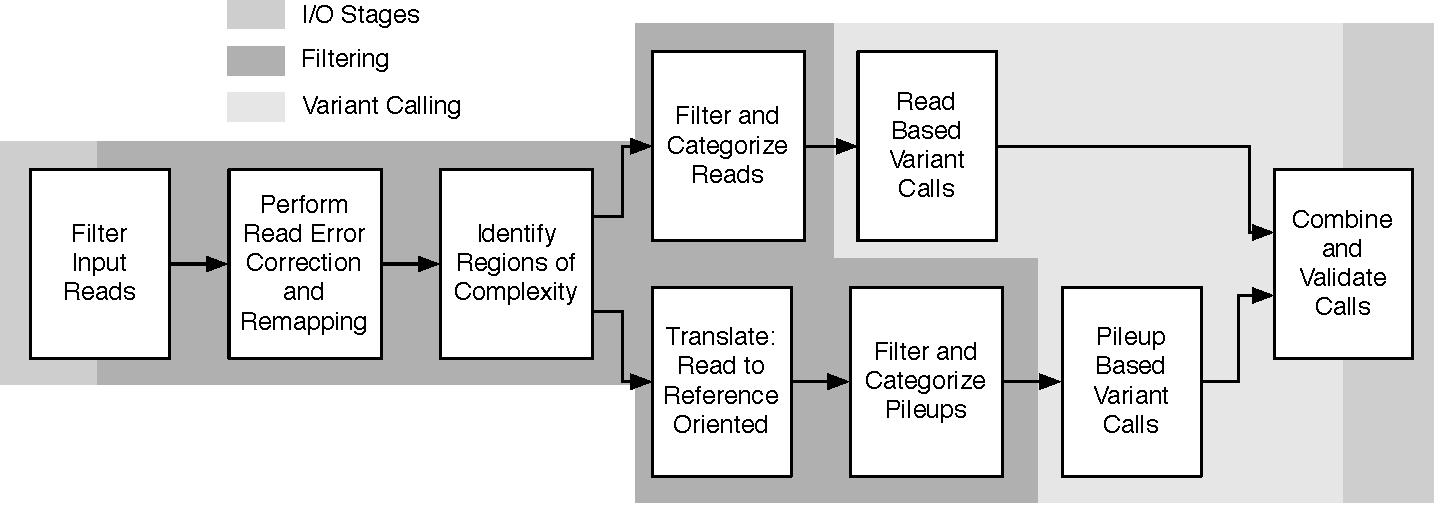
\includegraphics[width=0.8\linewidth]{avocado-architecture.pdf}
\end{center}
\caption{The architecture of the \texttt{avocado} pipeline}
\label{fig:avocado-architecture}
\end{figure}

In \texttt{avocado}, we support both read and reassembly based variant discovery, along with multiple statistical
methods for genotyping. Although the methods described in this thesis target human germline variant calling,
\texttt{avocado}'s local reassembly methods have been implemented so that they can support somatic variant
calling, and variant calling on polyploid genomes.

In this chapter, we first talk about \texttt{avocado}'s novel local reassembler, which is able to reduce the computational
complexity of local reassembly. This algorithmic reformulation also enables the reassembly of pooled/somatic and
polyploid samples, as it makes no assumptions about path count through the assembly graph. We then cover the
statistical models used for genotyping in \texttt{avocado}. A performance evaluation of \texttt{avocado} is provided
in~\S\ref{sec:variant-calling-performance}.

\section{Efficient Reassembly via Indexed \emph{de Bruijn} Graphs}
\label{sec:reference-threaded}

The accuracy of insertion and deletion~(INDEL) variant discovery has been improved by the development
of variant callers that couple local reassembly with haplotype-based statistical models to recover INDELs
that were locally misaligned~\cite{albers11}. Reassembly is a critical component of several prominent variant
callers such as the Genome
Analysis Toolkit's~(GATK) \texttt{HaplotypeCaller}~\cite{depristo11}, \texttt{Scalpel}~\cite{narzisi14}, and
\texttt{Platypus}~\cite{rimmer14}. Although haplotype-based methods have enabled more accurate INDEL
and single nucleotide polymorphism~(SNP) calls~\cite{bao14}, this accuracy comes at the cost of
end-to-end runtime~\cite{talwalkar14}. Several recent projects have been focused on improving
reassembly cost either by limiting the percentage of the genome that is reassembled~\cite{bloniarz14} or
by improving the performance of algorithms of the core algorithms used in local
reassembly~\cite{rimmer14}.

The performance issues seen in haplotype reassembly approaches derives from the high asymptotic
complexity of reassembly algorithms. Although specific implementations may vary slightly, a typical
local reassembler performs the following steps:

\begin{enumerate}
\item A \emph{de Bruijn} graph is constructed from the reads aligned to a region of the reference genome,
\item All valid paths~(\emph{haplotypes}) between the start and end of the graph are enumerated,
\item Each read is realigned to each haplotype, typically using a pair Hidden Markov Model~(HMM,
see~\cite{durbin98}),
\item A statistical model uses the read$\leftrightarrow$haplotype alignments to choose the haplotype pair
that most likely represents the variants hypothesized to exist in the region, 
\item The alignments of the reads to the chosen haplotype pair are used to generate statistics that are
then used for genotyping.
\end{enumerate}

In this paper, we focus on steps one through three of the local reassembly problem, as there is wide
variation in the algorithms used in stages four and five~(see~\S\ref{sec:background}). Stage one (graph
creation) has approximately $\mathcal{O}(r l_r)$ time complexity, and stage two (graph elaboration) has
$\mathcal{O}(h \max(l_h))$ time complexity.
The asymptotic time cost bound of local reassembly comes from stage three, where cost is $\mathcal{O}(h r l_r
\max(l_h))$, where $h$ is the number of haplotypes tested in this region\footnote{The number of
haplotypes tested may be lower than the number of haplotypes reassembled. Several tools
(see~\cite{depristo11,garrison12}) allow users to limit the number of haplotypes evaluated to improve
performance.}, $r$ is the number of reads aligned to this region, $l_r$ is the read length\footnote{For
simplicity, we assume constant read length. This is a reasonable assumption as many of the variant
callers discussed target Illumina reads that have constant length.}, and $\min(l_h)$ is the length of the
shortest haplotype that we are evaluating. This complexity comes from realigning $r$ reads to $h$
haplotypes, where realignment has complexity $\mathcal{O}(l_r l_h)$. We ignore the storage complexity of
reassembly here, but provide an extended
discussion of \emph{de Bruijin} graph complexity in~\S\ref{sec:background}.

In this paper, we introduce the \emph{indexed de Bruijn} graph and demonstrate how it can be used to
reduce the asymptotic complexity of reassembly. An \emph{indexed de Bruijn} graph is identical to a
traditional \emph{de Bruijn} graph, with one modification: when we create the graph, we annotate each
$k$-mer with the index position of that $k$-mer in the sequence it was observed in. This simple addition
enables the use of the \emph{indexed de Bruijn} graph for $\Omega(n)$ local sequence alignment with
canonical edit representations for most edits. This structure can be used for both sequence alignment and
assembly, and achieves a more efficient approach for variant discovery via local reassembly.

Current variant calling pipelines depend heavily on realignment based approaches for accurate
genotyping~\cite{li14}. Although there are several approaches that do not make explicit use of reassembly,
all realignment based variant callers use an algorithmic structure similar to the one described
in~\S\ref{sec:introduction}. In non-assembly approaches like \texttt{FreeBayes}~\cite{garrison12}, stages
one and two are replaced with a single step where the variants observed in the reads aligned to a given
haplotyping region are filtered for quality and integrated directly into the reference haplotype in that region.
In both approaches, local alignment errors~(errors in alignment \emph{within} this region) are corrected
by using a statistical model to identify the most likely location that the read could have come from, given
the other reads seen in this area.

Although the model used for choosing the best haplotype pair to finalize realignments to varies between
methods~(e.g., the GATK's \texttt{IndelRealigner} uses a simple log-odds model~\cite{depristo11}, while
methods like \texttt{FreeBayes}~\cite{garrison12} and \texttt{Platypus}~\cite{rimmer14} make use of richer
Bayesian models), these methods require an all-pairs alignment of reads to candidate
haplotypes. This leads to the runtime complexity bound of $\mathcal{O}(h r l_r \min(l_h))$ given
in~\S\ref{sec:introduction}, as we must realign $r$ reads to $h$ haplotypes, where the cost of realigning
one read to one haplotype is $\mathcal{O}(l_r \max(l_h))$, where $l_r$ is the read length~(assumed to be
constant for Illumina sequencing data) and $\max(l_h)$ is the length of the longest haplotype. Typically,
the data structures used for realignment~($\mathcal{O}(l_r \max(l_h))$ storage cost) can be reused.
These methods typically retain \emph{only} the best local realignment per read per haplotype, thus
bounding storage cost at $\mathcal{O}(h r)$.

For non-reassembly based approaches, the cost of generating candidate haplotypes is $\mathcal{O}(r)$,
as each read must be scanned for variants, using the pre-existing alignment. These variants are typically
extracted from the CIGAR string, but may need to be normalized~\cite{li14}. \emph{de Bruijn} graph based 
reassembly methods have similar $\mathcal{O}(r)$ time complexity for building the \emph{de Bruijn}
graph as each read must be sequentially broken into $k$-mers, but these methods have a different
storage cost. Specifically, storage cost for a \emph{de Bruijn} graph is similar to $\mathcal{O}(k
(l_{\text{ref}} + l_{\text{variants}} + l_{\text{errors}}))$, where $l_{\text{ref}}$ is the length of the reference
haplotype in this region, $l_{\text{variants}}$ is the length of true variant sequence in this region, 
$l_{\text{errors}}$ is the length of erroneous sequence in this region, and $k$ is the $k$-mer size. In
practice, we can approximate both errors and variants as being random, which gives $\mathcal{O}(k
l_{\text{ref}})$ storage complexity. From this graph, we must enumerate the haplotypes present in the
graph. Starting from the first $k$-mer in the reference sequence for this region, we perform a depth-first
search to identify all paths to the last $k$-mer in the reference sequence. Assuming that the graph is
acyclic~(a common restriction for local assembly, see~\S\ref{sec:limits-repeated-sequences}), we can
bound the best case cost of this search at $\Omega(h \min l_h)$.

The number of haplotypes evaluated, $h$, is an important contributor to the algorithmic complexity of
reassembly pipelines, as it sets the storage and time complexity of the realignment scoring phase, the
time complexity of the haplotype enumeration phase, and is related to the storage complexity of the
\emph{de Bruijn} graph. The best study of the complexity of assembly techniques was done by Kingsford
et al.~\cite{kingsford10}, but is focused on \emph{de novo} assembly and pays special attention to
resolving repeat structure. In the local realignment case, the number of haplotypes identified is determined
by the number of putative variants seen. We can na\"{i}vely model this cost with \eqref{eq:haplotypes},
where $f_v$ is the frequency with which variants occur, $\epsilon$ is the rate at which bases are
sequenced erroneously, and $c$ is the coverage (read depth) of the region.

\begin{align}
\label{eq:haplotypes}
h \sim f_v l_{\text{ref}} + \epsilon l_{\text{ref}} c
\end{align}

This model is na\"{i}ve, as the coverage depth and rate of variation varies across sequenced datasets,
especially for targeted sequencing runs~\cite{fang14}. Additionally, while the $\epsilon$ term models the
total number of sequence errors, this is not completely correlated with the number of \emph{unique}
sequencing errors, as sequencing errors are correlated with sequence context~\cite{depristo11}. Many
current tools allow users to limit the total number of evaluated haplotypes, or apply strategies to minimize
the number of haplotypes considered, such as filtering observed variants that are likely to be sequencing
errors~\cite{garrison12}, restricting realignment to INDELs~(\texttt{IndelRealigner},~\cite{depristo11}), or
by trimming paths from the assembly graph. Additionally, in an \emph{de Bruijn} graph, errors in the
first $k$ or last $k$ bases of a read will manifest as spurs~(see~\S\ref{sec:spurs}) and will not contribute paths through the graph. We provide~\eqref{eq:haplotypes} solely as a motivating
approximation, and hope to study these characteristics in more detail in future work.

\subsection{Formulation}
\label{sec:formulation}

To construct an \emph{indexed de Bruijn} graph, we start with the traditional formulation of a \emph{de
Brujin} graph for sequence assembly:

\begin{defn}[de Bruijn Graph]
\label{defn:dbg}
A de Bruijn graph describes the observed transitions between adjacent $k$-mers in a sequence. Each
$k$-mer $s$ represents a $k$-length string, with a $k - 1$ length prefix given by $\text{prefix}(s)$ and a
length 1 suffix given by $\text{suffix}(s)$. We place a directed edge ($\rightarrow$) from $k$-mer $s_1$ to
$k$-mer $s_2$ if $\text{prefix}(s_1)^{\{1, k - 2\}} + \text{suffix}(s_1) = \text{prefix}(s_2)$.
\end{defn}

Now, suppose we have $n$ sequences $\mathcal{S}_1, \dots, \mathcal{S}_n$. Let us assert that for each
$k$-mer $s \in \mathcal{S}_i$, then the output of function $\text{index}_i(s)$ is defined. This function
provides us with the integer position of $s$ in sequence $\mathcal{S}_i$. Further, given two $k$-mers
$s_1, s_2 \in \mathcal{S}_i$, we can define a distance function
$\text{distance}_i(s_1, s_2) = | \text{index}_i(s_1) - \text{index}_i(s_2) |$. To create an \emph{indexed
de Bruijn} graph, we simply annotate each $k$-mer $s$ with the $\text{index}_i(s)$ value for all
$\mathcal{S}_i, i \in \{1, \dots, n\}$ where $s \in \mathcal{S}_i$. This index value is trivial to log when
creating the original \emph{de Bruijn} graph from the provided sequences.

Let us require that all sequences $\mathcal{S}_1, \dots, \mathcal{S}_n$ are not repetitive, which implies
that the resulting \emph{de Bruijn graph} is acyclic. If we select any two sequences $\mathcal{S}_i$ and
$\mathcal{S}_j$ from $\mathcal{S}_1, \dots, \mathcal{S}_n$ that share at least two $k$-mers $s_1$ and
$s_2$ with common ordering~($s_1 \rightarrow \dots \rightarrow s_2$ in both $\mathcal{S}_i$ and
$\mathcal{S}_j$), the \emph{indexed de Bruijn} graph $G$ provides several guarantees:

\begin{enumerate}
\item If two sequences $\mathcal{S}_i$ and $\mathcal{S}_j$ share at least two $k$-mers $s_1$ and
$s_2$, we can provably find the maximum edit distance $d$ of the subsequences in $\mathcal{S}_i$ and
$\mathcal{S}_j$, and bound the cost of finding this edit distance at $\mathcal{O}(nd)$,\footnote{Here,
$n = \max(\text{distance}_{\mathcal{S}_i}(s_1, s_2), \text{distance}_{\mathcal{S}_j}(s_1, s_2))$.}
\item For many of the above subsequence pairs, we can bound the cost at $\mathcal{O}(n)$, \emph{and}
provide canonical representations for the necessary edits,
\item $\mathcal{O}(n^2)$ complexity is restricted to aligning the subsequences of $\mathcal{S}_i$ and
$\mathcal{S}_j$ that exist \emph{before} $s_1$ or \emph{after} $s_2$.
\end{enumerate}

Let us focus on cases 1 and 2, where we are looking at the subsequences of $\mathcal{S}_i$ and
$\mathcal{S}_j$ that are between $s_1$ and $s_2$. A trivial case arises when both $\mathcal{S}_i$ and
$\mathcal{S}_j$ contain an identical path between $s_1$ and $s_2$ (i.e.,
$s_1 \rightarrow s_n \rightarrow \dots \rightarrow s_{n + m} \rightarrow s_2$ and
$s_{n + k} \in \mathcal{S}_i \wedge s_{n + k} \in \mathcal{S}_j \forall k \in \{0, \dots , m\}$). Here, the
subsequences are clearly identical. This determination can be made trivially by walking from vertex $s_1$
to vertex $s_2$ with $\mathcal{O}(m)$ cost.

However, three distinct cases can arise whenever $\mathcal{S}_i$ and $\mathcal{S}_j$ diverge between
$s_1$ and $s_2$. For simplicity, let us assume that both paths are independent~(see
Definition~\ref{defn:path-independence}). These three cases correspond to there being either a canonical
substitution edit, a canonical INDEL edit, or a non-canonical (but known distance) edit between
$\mathcal{S}_i$ and $\mathcal{S}_j$.

\begin{defn}[Path Independence]
\label{defn:path-independence}
Given a non-repetitive \emph{de Bruijn} graph $G$ constructed from $\mathcal{S}_i$ and $\mathcal{S}_j$, we say
that $G$ contains independent paths between $s_1$ and $s_2$ if we can construct two subsets
$\mathcal{S}'_i \subset \mathcal{S}_i, \mathcal{S}'_j \subset \mathcal{S}_j$ of $k$-mers where $s_{i + n}
\in \mathcal{S}'_i \forall n \in \{0, \dots, m_i\}, s_{i + n - 1} \rightarrow s_{i + n} \forall n \in \{1, \dots, m_i\}$,
$s_{j + n} \in \mathcal{S}'_j \forall n \in \{0, \dots, m_j\}, s_{j + n - 1} \rightarrow s_{j + n} \forall n \in \{1,
\dots, m_j\}$, and $s_1 \rightarrow s_i, s_j; s_{i + m_i}, s_{j + m_j} \rightarrow s_2$ and $\mathcal{S}'_i
\bigcap \mathcal{S}'_j = \emptyset$, where $m_i = \text{distance}_{\mathcal{S}_i}(s_1, s_2)$, and $m_j =
\text{distance}_{\mathcal{S}_j}(s_1, s_2)$. This implies that the sequences $\mathcal{S}_i$ and
$\mathcal{S}_j$ are different between $s_1, s_2$,
\end{defn}

We have a canonical substitution edit if $m_i = m_j = k$, where $k$ is the $k$-mer size. Here, we can
prove that the edit between $\mathcal{S}_i$ and $\mathcal{S}_j$ between $s_1, s_2$ is a single base
substitution $k$ letters \emph{after} $\text{index}(s_1)$:

\begin{proof}[Proof regarding Canonical Substitution]
\label{proof:canonical-substitution}
Suppose we have two non-repetitive sequences, $\mathcal{S}_i'$ and $\mathcal{S}_j'$, each of length
$2k + 1$. Let us construct a \emph{de Bruijn} graph $G$, with $k$-mer length $k$. If each sequence begins with
$k$-mer $s_1$ and ends with $k$-mer $s_2$, then that implies that the first and last $k$ letters of
$\mathcal{S}_i'$ and $\mathcal{S}_j'$ are identical. If both subsequences had the same character at
position $k$, this would imply that both sequences were identical and therefore the two paths between
$s_1, s_2$ would not be independent~(Definition~\ref{defn:path-independence}). If the two letters are
different \emph{and} the subsequences are non-repetitive, each character is responsible for $k$
previously unseen $k$-mers. This is the only possible explanation for the two independent $k$ length
paths between $s_1$ and $s_2$.
\end{proof}

To visualize the graph corresponding to a substitution, take the two example sequences \texttt{CCACTGT}
and \texttt{CCAATGT}. These two sequences differ by a \texttt{C} $\leftrightarrow$ \texttt{A} edit at
position three. With $k$-mer length $k = 3$, this corresponds to the graph in Figure~\ref{fig:sne}.

\begin{figure}[h]
\begin{center}
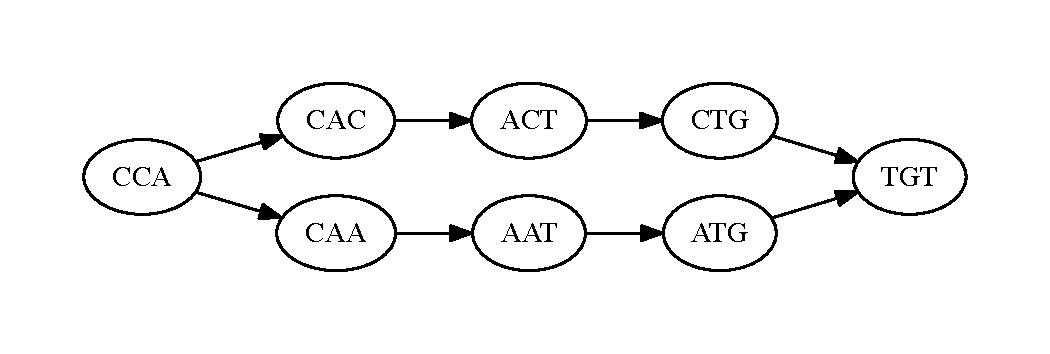
\includegraphics[width=0.5\linewidth, clip=true, trim=0 39 0 39]{graphs/sne.pdf}
\end{center}
\caption{Subgraph Corresponding To a Single Nucleotide Edit}
\label{fig:sne}
\end{figure}

If $m_i = k - 1, m_j \ge k$ or vice versa, we have a canonical INDEL edit (for convenience, we assume
that $\mathcal{S}_i'$ contains the $k - 1$ length path). Here, we can prove that there is a $m_j - m_i$
length insertion\footnote{This is equivalently a $m_j - m_i$ length deletion in $\mathcal{S}_i'$ relative to
$\mathcal{S}_j'$.} in $\mathcal{S}_j'$ relative to $\mathcal{S}_i'$, $k - 1$ letters \emph{after}
$\text{index}(s_1)$:

\begin{lemma}[Distance between $k$ length subsequences]
\label{lem:minimum-distance}
\emph{Indexed de Bruijn} graphs naturally provide a distance metric for $k$ length substrings. Let us construct an
\emph{indexed de Bruijn} graph $G$ with $k$-mers of length $k$ from a non-repetitive sequence $\mathcal{S}$.
For any two $k$-mers $s_a, s_b \in \mathcal{S}, s_a \ne s_b$, the
$\text{distance}_\mathcal{S}(s_a, s_b)$ metric is equal to $l_p + 1$, where $l_p$ is the length of the
path (in $k$-mers) between $s_a$ and $s_b$. Thus, $k$-mers with overlap of $k - 1$ have an edge
directly between each other ($l_p = 0$) and a distance metric of 1. Conversely, two $k$-mers that are
adjacent but not overlapping in $\mathcal{S}$ have a distance metric of $k$, which implies $l_p = k - 1$.
\end{lemma}

\begin{proof}[Proof regarding Canonical INDELs]
\label{proof:canonical-indels}
We are given a graph $G$ which is constructed from two non-repetitive sequences $\mathcal{S}_i'$ and
$\mathcal{S}_j'$, where the only two $k$-mers in both $\mathcal{S}_i'$ and $\mathcal{S}_j'$ are $s_1$
and $s_2$ and both sequences provide independent paths between $s_1$ and $s_2$. By
Lemma~\ref{lem:minimum-distance}, if the path from $s_1 \rightarrow \dots \rightarrow s_2 \in
\mathcal{S}_i'$ has length $k - 1$, then $\mathcal{S}_i'$ is a string of length $2k$ that is formed by
concatenating $s_1, s_2$. Now, let us suppose that the path from $s_1 \rightarrow \dots \rightarrow s_2
\in \mathcal{S}_j'$ has length $k + l - 1$. The first $l$ $k$-mers after $s_1$ will introduce a $l$ length
subsequence $\mathcal{L} \subset \mathcal{S}_j', \mathcal{L} \not\subset \mathcal{S}_i'$, and then the
remaining $k - 1$ $k$-mers in the path provide a transition from $\mathcal{L}$ to $s_2$. Therefore,
$\mathcal{S}_j'$ has length of $2k + l$, and is constructed by concatenating $s_1, \mathcal{L}, s_2$.
This provides a canonical placement for the inserted sequence $\mathcal{L}$ in $\mathcal{S}_j'$ between
$s_1$ and $s_2$.
\end{proof}

To visualize the graph corresponding to a canonical INDEL, take the two example sequences
\texttt{CACTGT} and \texttt{CACCATGT}. Here, we have a \texttt{CA} insertion after position two. With
$k$-mer length $k = 3$, this corresponds to the graph in Figure~\ref{fig:indel}.

\begin{figure}[h]
\begin{center}
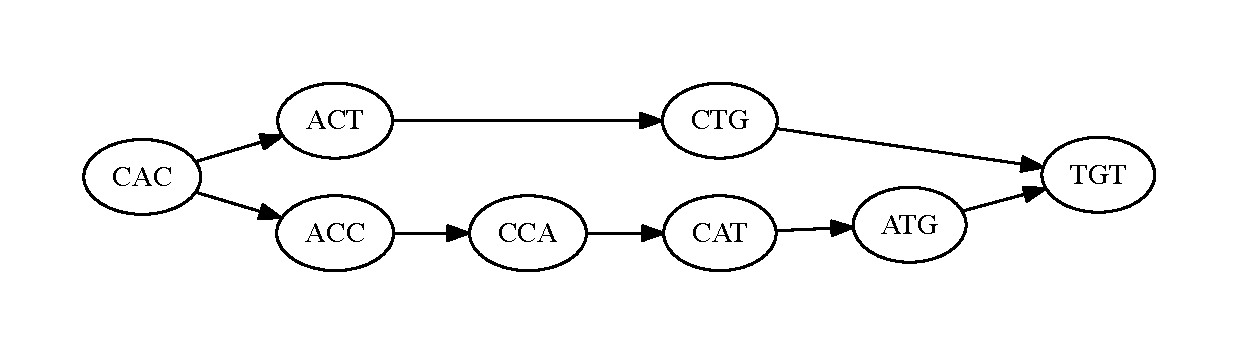
\includegraphics[width=0.5\linewidth, clip=true, trim=0 39 0 39]{graphs/indel.pdf}
\end{center}
\caption{Subgraph Corresponding To a Canonical INDEL Edit}
\label{fig:indel}
\end{figure}

Where we have a canonical allele, the cost of computing the edit is set by the need to walk the graph
linearly from $s_1$ to $s_2$, and is therefore $\mathcal{O}(n)$. However, in practice, we will see
differences that cannot be described as one of the earlier two canonical approaches. First, let us
generalize from the two above proofs: if we have two independent paths between $s_1, s_2$ in the
\emph{de Bruijn} graph $G$ that was constructed from $\mathcal{S}_i, \mathcal{S}_j$, we can describe
$\mathcal{S}_i$ as a sequence created by concatenating $s_1, \mathcal{L}_i, s_2$.\footnote{This
property holds true for $\mathcal{S}_j$ as well.} The canonical edits merely result from special cases:

\begin{itemize}
\item In a canonical substitution edit, $l_{\mathcal{L}_i} = l_{\mathcal{L}_j} = 1$.
\item In a canonical INDEL edit, $l_{\mathcal{L}_i} = 0, l_{\mathcal{L}_j} \ge 1$.
\end{itemize}

Conceptually, a non-canonical edit occurs when two edits occur within $k$ positions of each other. In
this case, we can trivially fall back on a $O(nm)$ local alignment algorithm~(e.g., a pairwise HMM or
Smith-Waterman, see~\cite{durbin98,smith81}), \emph{but} we only need to locally realign
$\mathcal{L}_i$ against $\mathcal{L}_j$, which reduces the size of the realignment problem. However, we
can further limit this bound by limiting the maximum number of INDEL edits to $d = | l_{\mathcal{L}_i} -
l_{\mathcal{L}_j} |$. This allows us to use an alignment algorithm that limits the number of INDEL
edits~(e.g., Ukkonen's algorithm~\cite{ukkonen85}). By this, we can achieve $O(n(d + 1))$ cost.

\subsection{Specialization for Local Reassembly}
\label{sec:local-reassembly}

As stated in~\S\ref{sec:formulation}, we have assumed that we want to find the edits between two or
more \emph{known} sequences. However, when performing local reassembly for variant discovery/calling,
our goal is to identify all possible variants and to associate probabilities to observations that contain these
variants. This hypothesized variants are generated by examining the reads aligned to the reference
at/near a given site.

However, we can adopt a ``pooled'' model that uses the \emph{indexed de Bruijn} graph to discover alternate
alleles without performing a search for all haplotypes. Here, we extract a substring $\mathcal{R}$ from a
reference assembly, corresponding to the subsection of that reference that we would like to reassemble.
Then, we create a pooled ``sequence'' $\mathcal{P}$, that is generated from the $k$-mers present in
the reads aligned to $\mathcal{R}$. However, since $\mathcal{P}$ is a composite of the pooled reads, we
cannot assign indices to $k$-mers in $\mathcal{P}$. Instead, we will rely wholly on the path length
properties demonstrated in~\S\ref{sec:formulation} and the indices of $k$-mers in $\mathcal{R}$ to
discover and anchor alleles. First, let us classify paths where $\mathcal{R}$ and $\mathcal{P}$ diverge
into two types:

\begin{itemize}
\item \textbf{Spurs:} A spur is a set $S$ of $n$ $k$-mers $\{s_1, \dots, s_n\}$ where either $s_1$ or
$s_n \in \mathcal{R}, \mathcal{P}$ and all other $k$-mers are $\not\in \mathcal{R}, \in \mathcal{P}$,
and where $s_i \rightarrow s_{i + 1} \forall i \in \{1, \dots, n - 1\}$. If $s_1 \in \mathcal{R}$, then $s_n$ must 
not have a successor. Alternatively, if $s_n \in \mathcal{R}$, than $s_1$ is required to not have a
predecessor.
\item \textbf{Bubbles:} A bubble is a set $S$ of $n$ $k$-mers $\{s_1, \dots, s_n\}$ where both $s_1$ and
$s_n \in \mathcal{R}, \mathcal{P}$ and all other $k$-mers are $\not\in \mathcal{R}, \in \mathcal{P}$, and
where $s_i \rightarrow s_{i + 1} \forall i \in \{1, \dots, n - 1\}$.
\end{itemize}

Currently, we disregard spurs. Spurs typically result from sequencing errors near the start or end of a
read. Additionally, given a spur, we cannot put a constraint on what sort of edit it may be from the
reference, which increases the computational complexity of processing the spur. We concede that this
may not be the best approach, and have included a longer discussion of the accuracy impact of this
decision, as well as options for processing spurs with an \emph{indexed de Bruijn} graph in~\S\ref{sec:spurs}.

We can elaborate the graph and identify variants by walking the graph from the first $k$-mer in
$\mathcal{R}$. Although haplotype elaboration algorithms have $\Omega(h \min l_h)$ cost~(see~\S\ref{sec:background}) where
$\min l_h$ is the length of the shortest haplotype and $h$ is the number of haplotypes described by the graph, we can limit our graph traversal
to have $\mathcal{O}(n)$ runtime cost where $n = V(G)$ by introducing a tail-recursive finite state machine~(FSM). Whenever we
reach a branch point in the graph, our FSM will push state onto a stack, which allows us---with a few
exceptions---to avoid making multiple traversals through a single $k$-mer in the graph. Our FSM has
the following states:

\begin{itemize}
\item \texttt{R}, \texttt{Reference}: We are on a run of $k$-mers that are in $\mathcal{R}$.
\item \texttt{A}, \texttt{Allele}: We are on a run of $k$-mers that have diverged off of the reference. We
have a divergence start point, but have not connected back to the reference yet. This could be either
a bubble or a spur. 
\item \texttt{C}, \texttt{ClosedAllele}: We were on a run of $k$-mers that had diverged off of the reference,
but have just reconnected back to the reference and now know the start and end positions~(in
$\mathcal{R}$) of the bubble, as well as the non-reference sequence and length of the bubble.
\end{itemize}

We allow the FSM to make the following state transitions, which are depicted in Figure~\ref{fig:fsm}:

\begin{itemize}
\item \texttt{R} $\rightarrow$ \texttt{R}: We are continuing along a reference run.
\item \texttt{R} $\rightarrow$ \texttt{A}: We were at a $k$-mer $\in \mathcal{R}$, and have seen a branch
to a $k$-mer $\not\in \mathcal{R}$.
\item \texttt{A} $\rightarrow$ \texttt{A}: We are continuing along a non-reference run.
\item \texttt{A} $\rightarrow$ \texttt{C}: We were on a non-reference run, and have just connected back to
a reference $k$-mer.
\item \texttt{C} $\rightarrow$ \texttt{R}: We have just closed out an allele, and are back at a $k$-mer
$\in \mathcal{R}$.
\end{itemize}

\begin{figure}[h]
\begin{center}
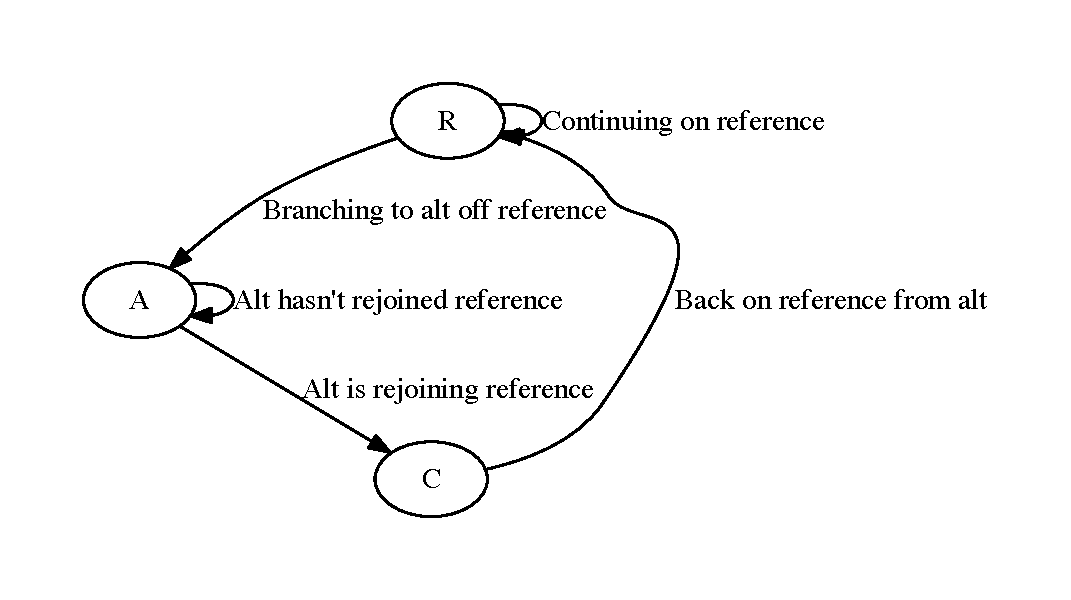
\includegraphics[width=0.5\linewidth, clip=true, trim=0 39 0 39]{graphs/fsm.pdf}
\end{center}
\caption{Finite State Machine for Pooled vs. Reference Assembly}
\label{fig:fsm}
\end{figure}

We initialize the state machine to \texttt{R}, and start processing with the first $k$-mer from $\mathcal{R}$.
Per $k$-mer, we evaluate the possible state transitions of each successor $k$-mer. If the set of successor
$k$-mers contains a single $k$-mer, we continue to that state. If the successor set contains multiple
$k$-mers, we choose a successor state to transition to, and push the branch context of all other
successor states onto our stack. If the successor set is empty, we pop a branch context off of the stack,
and switch to that context. We stop once we reach a $k$-mer whose successor set is empty, \emph{and}
our branch context stack is empty.

The implementation of the \texttt{R} and \texttt{A} states largely amount to bookkeeping. In the \texttt{R}
state, we must track the current position in $\mathcal{R}$, and in \texttt{A}, we must record where we
branched off of $\mathcal{R}$, and $\mathcal{L}'$, the bases we have seen since we
branched\footnote{Although we are processing $k$-mers, we only need to reconstruct the sequence that
the $k$-mers are describing by taking the first base from each successive $k$-mer.} off of $\mathcal{R}$.
If we are in the \texttt{A} state and walk to a $k$-mer $\in \mathcal{R}$, we then transition into the
\texttt{C} state. Using the positions of our branch point and the current $k$-mer in $\mathcal{R}$, we are
able to calculate the length of the reference path via Lemma~\ref{lem:minimum-distance}, while the length
of the non-reference path is given by $l_{\mathcal{L}'}$. The edited sequence $\mathcal{L}$ present
between the branch point and the current $k$-mer is given by trimming the first $k - 1$ bases from
$\mathcal{L}'$. If we have a non-canonical edit, or a deletion in $\mathcal{P}$ relative to $\mathcal{R}$,
we can look these bases up by indexing into $\mathcal{R}$.

To improve computational efficiency, we should emit statistics for genotyping \emph{while} traversing the graph. By doing 
this, we can eliminate the need for realignment in haplotype reassembly. Since we have constructed a
graph where every $k$-mer is anchored to a reference position or to a position in a variant, or is in a spur,
if we log several statistics when processing reads from $\mathcal{P}$, we can directly emit the probability
observations that support a reference base or a variant allele. Although the relevant statistics vary
between different variant calling/genotyping algorithms, common statistics include base and mapping
quality, as well as strand of the observation. Additionally, genotyping algorithms that incorporate phasing
may want to identify observations that came from the same allele. These statistics can be logged when
chopping the reads in $\mathcal{P}$ into $k$-mers at a low cost.

As noted earlier in this section, we normally do \emph{not} need to retrace through any $k$-mers in the
graph when processing the graph. However, we may need to retrace $k$-mers if we have overlapping
variants. For example, take the reference string \texttt{ACTGCCGTCT}, the SNV \texttt{ACTGCAGTCT},
and the complex variant \texttt{ACTGCAAGTCT}\footnote{At \texttt{CCG}, we have inserted an \texttt{A}
between the two \texttt{C}s, and changed the second \texttt{C} $\rightarrow$ \texttt{A}. Alternatively, this
can be described as a deletion of the second \texttt{C} and an insertion of \texttt{AA} between
\texttt{CG}.}. For $k = 4$, both variants share the 4-mer \texttt{AGTC}, but both take independent paths
from the reference 4-mer \texttt{CTGC} to \texttt{AGTC}. In this case, we need to walk \texttt{AGTC} twice.

\section{Statistical Models for Genotyping}
\label{sec:statistical-genotyping}

\texttt{avocado} supports two germline genotyping models. The first model is a traditional genotyping model
based off of the biallelic genotyping model from \texttt{samtools}~\cite{li11snp}. The second model is a novel
monoallelic model that is built on top of an \emph{allele graph}. The biallelic model assumes per site independence,
while the monoallelic model is a haplotyping model that jointly scores sites within a single region. Both models
can be incorporated into a joint variant calling approach, where we integrate over multiple samples to update the
probabilities of a genotype call.

\subsection{Biallelic Genotyping Model}
\label{sec:biallelic-genotyping}

The biallelic genotyping model in \texttt{avocado} is derived closely from the biallelic genotyping model used in the
\texttt{samtools mpileup} variant caller~\cite{li11snp}. However, we make several modifications. First, we apply
a windowing approach to unify ``complex'' events. Second, we operate solely in log space. This is done in order to
avoid the underflow issues discussed in \S2.3.6 of Li 2011~\cite{li11snp}.

\subsubsection{Windowing Algorithm}
\label{sec:windowing}

The site independence assumption in \texttt{samtools mpileup} serves as a simplification for the statistical approaches
that follow, but can be a source of error in the presence of INDELs and other complex events. As asserted earlier in
this section, we believe that we can arrive at a canonical INDEL alignment via local reassembly. This canonicalization
should resolve issues due to read evidence for an INDEL allele being misaligned across multiple reads. However,
even after realignment, we cannot guarantee that we have observed the same alleles across \emph{all} samples, nor
can we guarantee that all alleles are at a single site on the reference genome. This is trivial to note: all deletions cover
a \emph{region} of the reference genome, not a single site. As such, grouping together alleles by start position is not
sufficient for correctness. While performing a coordinate space self-join---as supported in \texttt{ADAM}---would be
sufficient for \emph{correctness}, it would not be performant due to the number of observations being scored in a large
dataset. Instead, we apply the sweeping window approach given in Algorithm~\ref{alg:window-observations}.

\begin{algorithm}
\caption{Open Windows for Site Observations}
\label{alg:window-observations}
\begin{algorithmic}
\STATE $observations \leftarrow$ the set of allele observations
\STATE $contigs \leftarrow$ a description of the reference genome assembly
\STATE $observations \leftarrow observations$.repartitionAndSortWithinPartition($contigs$)
\STATE $sites \leftarrow \emptyset$
\FOR{$partition \in observations$}
\STATE $windowStart \leftarrow partition$.head.start
\STATE $windowEnd \leftarrow partition$.head.end
\STATE $site \leftarrow \emptyset$
\FOR{$observation \in partition$}
\IF{$windowEnd <= observation$.start}
\STATE $site = \{observation\}$)
\ELSE
\STATE $window \leftarrow [windowStart, windowEnd)$
\STATE $sites$.append($(window, site)$)
\STATE $site$.append($observation$)
\ENDIF
\ENDFOR
\IF{$sites \ne \emptyset$}
\STATE $window \leftarrow [windowStart, windowEnd)$
\STATE $sites$.append($(window, site)$)
\ENDIF
\ENDFOR
\RETURN $sites$
\end{algorithmic}
\end{algorithm}

This algorithm maintains an open window that it uses to group together all observations that are in the window. It is
worth noting that this is different from a self-join or a groupBy. Specifically, we group all observations into the smallest
possible region that could fully contain those observations. If multiple observations from the same read are grouped
together, we then combine the statistics from those observations, weighted by the number of bases from the read
contributing to each respective observation.

\subsubsection{Statistical Model}
\label{sec:genotyping-model}

The biallelic genotyping model in \texttt{avocado} is derived directly from \texttt{mpileup}~\cite{li11snp}, except with a
translation to log space. We calculate log likelihoods from the site observations, and use the major allele
frequency~(MAF)\footnote{The frequency of the reference allele as observed at this site across all samples.} as a prior
when normalizing. We use equation~\eqref{eq:likelihood} to calculate the log likelihood of the genotype state at a site.
Terms used in the equation are defined in Table~\ref{tab:likelihood-terms}.

\begin{align}
\label{eq:likelihood}
l(g) &= -k \log m + \sum_{i = 1}^{j} \log(\epsilon_i (m - g) + (1 - \epsilon_i) g) + \sum_{i = j + 1}^{k} \log(\epsilon_i g + (1 - \epsilon_i) (m - g))
\end{align}

\begin{table}[h]
\begin{center}
\caption{Equation~\eqref{eq:likelihood} Terms}
\label{tab:likelihood-terms}
\begin{tabular}{| c | l |}
\hline
Term & Definition \\
\hline
\hline
$m$ & The copy number of the site. \\
$g$ & The \emph{genotype state}, or number of reference alleles. \\
$j$ & Reads $\in k$ that support the reference allele. \\
$k$ & The total number of reads at the site \\
$\epsilon_i$ & The probability that observation $i$ was in error. \\
\hline
\end{tabular}
\end{center}
\end{table}

We estimate the MAF via expectation-maximization. Our update equation for $n$ samples is given in
Equation~\ref{eq:em}. $c_s$ represents the contribution of sample $s$ to the MAF, and $p_s(g l_{\text{MAF}})$ is the
probability of genotype state $g$ for sample $s$, given $l_{\text{MAF}}$. The MAF is treated as a binomial prior.

\begin{align}
\label{eq:em}
l_{\text{MAF}} &= s(c_1, \dots, c_n) \\
c_s &= s(n_{s, i}, \dots) - s(d_{s, i}, \dots), i \in \{0, \dots, g\} \\
n_{s, i} &= p_s(i | l_{\text{MAF}}) + \log i \\
d_{s, i} &= p_s(i | l_{\text{MAF}}) \\
\label{eq:log-sum}
s(l_1, l_2) &= l_1 + \log(1 + e^\frac{l_2}{l_1}) \\
\label{eq:log-recursive-sum}
s(l_1, l_2, \dots , l_n) &= s(l_1, s(l_2, s( \dots s(l_{n - 1}, l_n)))) \\
\end{align}

We use Equation~\eqref{eq:log-sum} is a numerically stable algorithm for adding two log values to each other and
returning a log result. This equation is from Durbin et al~\cite{durbin98}. To sum together an array of log values, we
compose Equation~\eqref{eq:log-sum} recursively into Equation~\eqref{eq:log-recursive-sum}. In practice, to improve
numerical stability we sort the array before performing the recursive sum.

\subsection{Monoallelic Genotyping Model}
\label{sec:monoallelic-genotyping}

In an alternative formulation, we can consider the observed alleles as a directed graph. We refer to this as an
\emph{allele graph}, and this serves as a basis on which we can apply probabilistic graphical modeling techniques.
To construct the graph, each allele is given a node. We connect two nodes with an edge if and only if a read is observed
to cover both nodes. In Figure~\ref{fig:alleles}, we present a sequence where the reference is
\texttt{ACCCTATCGCTCACA}. Evidence of a \texttt{C} $\rightarrow$ \texttt{G} single nucleotide
polymorphism~(SNP) is present at position 3, and evidence of a deletion of bases 8--9 (\texttt{GC}) is
present.

\begin{figure}[h]
\begin{center}
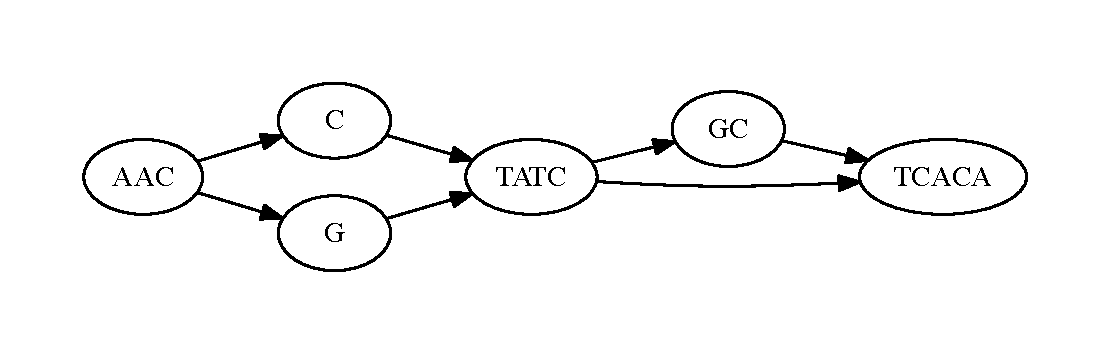
\includegraphics[width=0.4\linewidth]{graphs/alleles.pdf}
\end{center}
\caption{Allele Graph}
\label{fig:alleles}
\end{figure}

Between two nodes, we can define a conditional probability $P(x = X | y = Y)$, which is the probability that
node $x$ has copy number $X$ and node $y$ has copy number $Y$:

\begin{align}
\label{eq:cond-prob}
P(x = X | y = Y) = \frac{1}{Y^k}\prod_{i = 1}^{j} ( X P_i + (Y - X) (1 - P_i)) \prod_{i = j + 1}^{k} ((Y - X) P_i + X P_i )
\end{align}

In equation~\eqref{eq:cond-prob}, we have the following terms:

\begin{table}[h]
\begin{center}
\caption{Equation~\eqref{eq:cond-prob} Terms}
\label{tab:cond-prob-terms}
\begin{tabular}{| c | l |}
\hline
Term & Definition \\
\hline
\hline
$X$ & The copy number of the $x$ allele. \\
$Y$ & The copy number of the $y$ allele. \\
$k$ & The number of reads in the $y$ allele that span \emph{any} allele in the $x$ direction. \\
$i$ & Reads $\in k$ that support a transition from $y \rightarrow x$. \\
$j$ & Reads $\in k$ that do \emph{not} support a transition from $y \rightarrow x$. \\
$P_i$ & The probability that read $i$ supports a transition from $y \rightarrow x$. \\
\hline
\end{tabular}
\end{center}
\end{table}

While equation~\eqref{eq:cond-prob} is useful, it only covers a single, uninteresting scenario. Specifically, it does not
cover the case where we have a fork in the graph. In this case, we can define a further equation:

\begin{align}
\label{eq:multi-cond}
P(x = X | y_1 = Y_1, \dots, y_n = Y_n) = \sum_{X_1 + \dots + X_n = X, X_i \ge 0} P(X_1, \dots, X_n | \frac{Y_1}{\sum Y}, \dots, \frac{Y_n}{\sum Y}) \prod_{i = 1}^{n} P(x = X | y_i = Y_i)
\end{align}

where $P(X_1, \dots, X_n | \frac{Y_1}{\sum Y}, \dots, \frac{Y_n}{\sum Y})$ is multinomial.

With equation~\eqref{eq:multi-cond} defined, we can calculate full conditional probabilities for all nodes in the graph. Once
we've done this, we can marginalize out all the conditional probabilities by running belief propagation from the root of the
graph~\cite{pearl86}. We do make a single assertion here: specifically, we assume that all spurs are trimmed from the
allele graph, and we have a clearly defined ``root'' for the graph. This is easy to provide in our local assembly scenario,
where we have a clearly defined start to the active region for reassembly; for \emph{de novo} assembly, we may be able to
define this by finding a cut of the graph that minimizes a certain function. 

\chapter{Performance and Accuracy Analysis}

Thus far, we have discussed ways to improve the performance of scientific workloads that are
being run on commodity MapReduce systems by rethinking how we decompose and build algorithms.
In this section, we review the improvements in performance that we are able to unlock. We achieve
near-linear speedup across 128 nodes for a genomics workload, and achieve a $3\times$ performance
improvement over the current best MPI-based system for the Montage astronomy application.
Additionally, both systems achieve 25-50\% compression over current file formats when storing to disk.

\section{Genomics Workloads}
\label{sec:genomics-performance}

Table~\ref{tab:overview} previews our performance versus current systems. The tests in this table are run on the
high coverage \texttt{NA12878} full genome BAM file that is available from the 1000 Genomes
project.\footnote{The file used for these experiments can be found on the
1000 Genomes ftp site, \url{ftp.1000genomes.ebi.ac.uk} in directory 
\texttt{/vol1/ftp/data/NA12878/high\_coverage\_alignment/} for NA12878.} These tests have been run on the EC2 cloud, using the instance types listed in
Table~\ref{tab:machines}. We compute the cost of running each experiment by multiplying the number of instances
used by the total wall time for the run and by the cost of running a single instance of that type for an hour, which is
the process Amazon uses to charge customers.

\begin{table}[h]
\caption{Summary Performance on NA12878}
\label{tab:overview}
\begin{center}
\begin{tabular}{ l c c c }
\hline
\multicolumn{4}{c}{\textbf{\textit{Sort}}} \\
\textbf{Software} & \textbf{EC2 profile} & \textbf{Time} & \textbf{Cost} \\
\hline
Picard & 1 \texttt{hs1.8xlarge} & 17h 44m & \$81.57 \\
ADAM & 1 \texttt{hs1.8xlarge} & 8h 56m & \$41.09 \\
ADAM & 128 \texttt{m2.4xlarge} & 9m & \$31.49 \\
\hline
\multicolumn{4}{c}{\textbf{\textit{Mark Duplicates}}} \\
\textbf{Software} & \textbf{EC2 profile} & \textbf{Time} & \textbf{Cost} \\
\hline
Picard & 1 \texttt{hs1.8xlarge} & 20h 22m & \$93.68 \\
ADAM & 1 \texttt{hs1.8xlarge} & 9h & \$41.40 \\
ADAM & 128 \texttt{m2.4xlarge} & 19m & \$64.48 \\ 
\hline
\multicolumn{4}{c}{\textbf{\textit{BQSR}}} \\
\textbf{Software} & \textbf{EC2 profile} & \textbf{Time} & \textbf{Cost} \\
\hline
GATK & 1 \texttt{hs1.8xlarge} & 31h 18m & \$143.98 \\
ADAM & 1 \texttt{hs1.8xlarge} & 34h & \$156.40 \\
ADAM & 128 \texttt{m2.4xlarge} & 54m & \$188.93 \\
\hline
\multicolumn{4}{c}{\textbf{\textit{INDEL Realignment}}} \\
\textbf{Software} & \textbf{EC2 profile} & \textbf{Time} & \textbf{Cost} \\
\hline
GATK & 1 \texttt{hs1.8xlarge} & 42h 49m & \$196.88 \\
ADAM & 1 \texttt{hs1.8xlarge} & 12h 58m & \$82.80 \\
ADAM & 128 \texttt{m2.4xlarge} & 24m & \$83.97 \\
\hline
\multicolumn{4}{c}{\textbf{\textit{Flagstat}}} \\
\textbf{Software} & \textbf{EC2 profile} & \textbf{Time} & \textbf{Cost} \\
\hline
SAMtools & 1 \texttt{hs1.8xlarge} & 25m 24s & \$1.95 \\
ADAM & 1 \texttt{hs1.8xlarge} & 7m 4s & \$1.95 \\
ADAM & 128 \texttt{cr1.8xlarge} & 1m 53s & \$5.35 \\
\hline
\end{tabular}
\end{center}
\end{table}

Table~\ref{tab:machines} describes the instance types. Memory capacity is reported in Gibibytes~(GiB).
Storage capacities are not reported in this table because disk
capacity does not impact performance, but the number and type of storage drives is reported because
aggregate disk bandwidth does impact performance. In our tests, the \texttt{hs1.8xlarge} instance is
chosen to represent a workstation. Network bandwidth is constant across all instances.

\begin{table}[h]
\caption{AWS Machine Types}
\label{tab:machines}
\begin{center}
\begin{tabular}{ l c l }
\hline
\textbf{Machine} & \textbf{Cost} & \textbf{Description} \\
\hline
\hline
\texttt{hs1.8xlarge} & \$4.60/hr & 16 proc, 117GiB RAM, 24$\times$ HDD \\
\texttt{m2.4xlarge} & \$1.64/hr & 8 proc, 68.4GiB RAM, 2$\times$ HDD \\
\hline
\end{tabular}
\end{center}
\end{table}

As can be seen from these results, our pipeline is at best three times faster than current pipelines when running
on a single node; at worst, we are approximately at parity. Additionally, \texttt{ADAM} achieves speedup that is
close to linear. This point is not clear from Table~\ref{tab:overview}, as we change instance types when also
changing the number of instances used. Figure~\ref{fig:speedup} presents speedup plots for the NA12878 high
coverage genome.

\begin{figure}[h]
\begin{center}
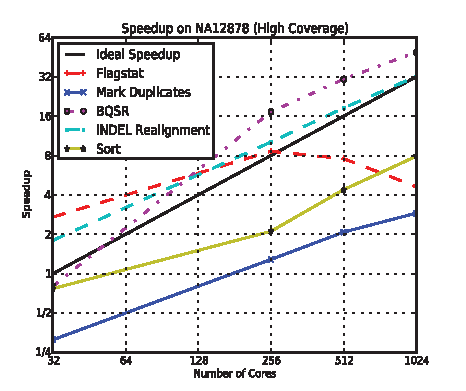
\includegraphics[width=0.99\linewidth]{graphs/speedup_na12878.pdf}
\end{center}
\caption{Speedup on NA12878}
\label{fig:speedup}
\end{figure}

When testing on NA12878, we achieve linear speedup out through 1024 cores; this represents 128
\texttt{m2.4xlarge} nodes. In this test, our performance is limited by several factors:

\begin{itemize}
\item Although columnar stores have very high read performance, their write performance is low. Our
tests exaggerate this penalty; since a variant calling pipeline will consume a large read file, but then output a
variant call file that is approximately two orders of magnitude smaller, the write penalty will be reduced. In
practice, we also use in-memory caching to amortize write time across several stages.
\item Additionally, for large clusters, straggler elimination is an issue. However, we have made optimizations to
both the \texttt{Mark Duplicates} and \texttt{INDEL Realignment} code to eliminate stragglers by randomly
rebalancing reads that are unmapped/do not map to a target across partitions.
\end{itemize}

We do note that the performance of \texttt{flagstat} degrades going from 32 to 128 \texttt{m2.4xlarge} nodes.
It is worth noting that \texttt{flagstat} executes in one minute on 32 nodes. By increasing the number of machines
we use to execute this query, we increase scheduling overhead, which leads to degraded
performance.\footnote{While we
have tested against the SAMtools/Picard/GATK pipeline, we do note that new implementations have come out
recently~(e.g., SAMBAMBA and SAMBLASTER~\cite{faust14}) that focus on fast duplicate marking. We have not
compared to them due to time limitations, but will compare to them in a later revision of this paper.}

\section{Column Store Performance}
\label{sec:column-store-perf}

Earlier in this paper, we motivated the use of a column store as it would allow us to better push processing to
the data. Specifically, we can use predicate pushdown and projections to minimize the amount of I/O that we
perform. Additionally, column stores provide compressed storage, which allows us to minimize both the required
I/O bandwidth and space on disk. In this section, we'll look at the performance that our columnar store achieves
in terms of read performance and compression. We will not look extensively at write performance; for genomic
data, write performance is not a bottleneck because our workflow computes a \emph{summarization} of a large
dataset. As a result, our output dataset tends to be O(100 MB) while our input dataset is in the range of
O(10 GB)--O(100GB).

\subsection{Compression}
\label{sec:compression}

The Parquet columnar store~\cite{parquet} supports several compression features. Beyond traditional block-level
compression, Parquet supports run length encoding for repeated values, dictionary encoding, and delta
encoding. Currently, we make use of run length encoding to compress highly repeated metadata value,
and dictionary encoding to compress fields that can take a limited range of values. Dictionary encoding provides
substantial improvements for genomic data; specifically, the majority of genomic sequence data can be
represented with three bits per base.\footnote{Although DNA only contains four bases (A, C, G, and T),
\emph{sequenced} DNA uses disambiguation codes to indicate that a base was read in error. As a result, we
cannot achieve the ideal two-bits per base.} This is an improvement over our in-memory string representation
which allocates a byte per base.

In Table~\ref{tab:genomic-compression}, we look at the compression we achieve on the \texttt{NA12878}
and \texttt{HG00096}\footnote{A link to the \texttt{NA12878} dataset was provided earlier in this paper. The
\texttt{HG00096} dataset is available from \url{ftp.1000genomes.ebi.ac.uk} in directory 
\texttt{/vol1/ftp/data/HG00096/alignment/}.} human genome sequencing samples. We compare against the
GZIP compressed BAM~\cite{li09} format, and the CRAM format~\cite{fritz11}. We achieve approximately a
$1.25\times$ improvement in storage. This is not as impressive as the result achieved by the CRAM project,
but the CRAM project applies specific compression techniques that make use of the read alignment. Specifically,
CRAM only stores the read bases that \emph{do not} appear in the reference genome. As we only expect a
genomic variant at one in every 1000 bases, and a read error at one in every 50 bases, this allows them to
achieve significant compression of the sequenced bases.

\begin{table}[h]
\caption{Genomic Data Compression}
\label{tab:genomic-compression}
\begin{center}
\begin{tabular}{ l c c }
\hline
\multicolumn{3}{c}{\textbf{\texttt{NA12878}}} \\
\textbf{Format} & \textbf{Size} & \textbf{Compression} \\
\hline
\hline
BAM & 234 GB & --- \\
CRAM & 112 GB & 2.08$\times$ \\
Parquet & 185 GB & 1.26$\times$ \\
\hline
\multicolumn{3}{c}{\textbf{\texttt{HG00096}}} \\
\textbf{Format} & \textbf{Size} & \textbf{Compression} \\
\hline
\hline
BAM & 14.5 GB & --- \\
CRAM & 3.6 GB & 4.83$\times$ \\
Parquet & 11.4 GB & 1.27$\times$ \\
\hline
\end{tabular}
\end{center}
\end{table}

For genomic datasets, our compression is limited by the sequence and base quality fields, which respectively
account for approximately 30\% and 60\% of the space spent on disk. Quality scores are difficult to compress
because they are high entropy. We are currently looking into computational strategies to address this problem;
specifically, we are working to probabilistically estimate the quality scores \emph{without} having observed quality
scores. This would be performed via a process that is similar to the base quality score recalibration algorithm
presented earlier in this paper.

\subsection{Horizontal Scalability}
\label{sec:horizontal-scalability}

The representation Parquet uses to store data to disk is optimized for horizontal scalability in several ways.
Specifically, Parquet is implemented as a hybrid row/column store where the whole set of records in a dataset
are partitioned into row groups which are then serialized in a columnar layout. This provides us with two additional
benefits:

\begin{enumerate}
\item We are able to perform parallel access to Parquet row groups without consulting metadata or checking for
a file split.
\item Parquet achieves very even balance across partitions. On the \texttt{HG00096} dataset, the average
partition size was 105 MB with a standard deviation of 7.4 MB. Out of the 116 partitions in the file, there is only
one partition whose size is not between 105--110MB.
\end{enumerate}

Parquet's approach is preferable when compared to Hadoop-BAM~\cite{niemenmaa12}, a project that supports
the direct usage of legacy BAM files in Hadoop. Hadoop-BAM must pick splits, which adds non-trivial overhead.
Additionally, once Hadoop-BAM has picked a split, there is no guarantee that the split is well placed. It is only
guaranteed that the split position will not cause a \emph{functional error}.

\subsection{Projection and Predicate Performance}
\label{sec:projection-predicate-performance}

We use the \texttt{flagstat} workload to evaluate the performance of predicates and projections in Parquet.
We define three projections and four predicates, and test all of these combinations. In addition to projecting the
full schema~(see Appendix~\ref{sec:genomics-schema}), we also use the following two projections:

\begin{enumerate}
\item We project the read sequence \emph{and} all of the flags (40\% of data on disk).
\item We only project the flags (10\% of data on disk).
\end{enumerate}

Beyond the null predicate (which passes every record), we evaluate the following three predicates:

\begin{enumerate}
\item We pass only uniquely mapped reads (99.06\% of reads).
\item We pass only the first pair in a paired end read (50\% of reads).
\item We pass only \emph{un}mapped reads (0.94\% of reads).
\end{enumerate}

Our performance is documented in Table~\ref{tab:ppp}. Projections are arranged in the columns of the table
while predicates are assigned to rows.

\begin{table}[h]
\caption{Predicate/Projection Speedups}
\label{tab:ppp}
\begin{center}
\begin{tabular}{ l | c c c c }
\hline
& 0 & 1 & 2 \\
\hline
\hline
0 & --- & 1.7 & 1.9 \\
1 & 1.0 & 1.7 & 1.7 \\
2 & 1.3 & 2.2 & 2.6 \\
3 & 1.8 & 3.3 & 4.4 \\
\hline
\end{tabular}
\end{center}
\end{table}

We achieve a $1.7\times$ speedup by moving to a projection that eliminates the deserialization of our most
complex field~(the quality scores that consume 60\% of space on disk), while we only get a $1.3\times$
performance improvement when running a predicate that filters 50\% of records. This can be partially attributed
to overhead from predicate pushdown; we must first deserialize a column, process the filter, and then read all
records who passed the pushdown filter. If we did not perform this step, we could do a straight scan over all of
the data in each partition.

\section{Variant Calling Performance}
\label{sec:variant-calling-performance}

Analysis of \texttt{avocado} to be added at a later date.

\chapter{Conclusion}

\section{Discussion}
\label{sec:discussion}

\section{Future Work}
\label{sec:future-work}

Our genomics work leverages columnar storage to improve performance and compression of data on disk,
with special emphasis on repetitive fields that can be run length encoded. While this improves
disk performance, it has the side effect of making data consume significantly more space in memory
than on disk. We are currently investigating techniques that leverage the immutability of data in our
applications to reduce memory consumption. We have changed Parquet and Avro's deserialization codec
to reuse allocated objects. For every value that is RLE'd, we only allocate the value once in memory. We
then share the value across all records which contained that value. This is especially important since we
maintain a lot of string metadata which is RLE'd on disk.

It is worth noting that there are many significant scientific applications (such as genome
assembly) that are expressed as traversal over graphs. Recent work by Simpson et al~(ABySS,
\cite{simpson09}) and Georganas et al~\cite{georganas14} has focused on using MPI
or Unified Parallel C~(UPC) to implement their own distributed graph traversal. Both systems
find that synchronization via message passing is a significant cost; specifically, the ABySS assembler
experiences scaling problems because it thrashes portions of the graph across nodes during traversal.
By building our system using Spark, we are able to leverage the GraphX processing library~\cite{gonzalez14,
xin13}. We are in the process of developing a genome assembler using this library system, and
believe that we can achieve improved performance through careful graph partitioning. This partitioning involves
algorithmic changes to the graph creation and traversal phases to bypass ``knotted'' sections of the
graph that correspond to highly repetitive areas of the genome, which cause the major performance
issues in MPI based assemblers.

\section{Conclusion}
\label{sec:conclusion}

In this paper, we have advocated for an architecture for decomposing the implementation of a scientific
system, and then demonstrated how to efficiently implement genomic and astronomy processing pipelines using
the open source Avro, Parquet, and Spark systems~\cite{avro, parquet, zaharia10}. We have identified common
characteristics across scientific systems, like the need to run queries that touch slices of datasets and the need
for fast access to metadata. We then enforced data independence through a layering model that uses a schema
as the ``narrow waist'' of the stack, and used optimizations to make common, coordinate-based processing
fast. By using Parquet, a modern columnar store, we use predicates and projections to minimize I/O, and are able
to denormalize our schemas to improve the performance of accessing metadata.

By rethinking the architecture of scientific data management systems, we have been able to achieve
22--$131\times$ performance improvements over conventional genomics processing systems, along with linear
strong scaling and a $2\times$ cost improvement. On the astronomy workload, we achieve speedup between
2.8--$8.9\times$ speedup over the current best MPI-based solution at various scales. By applying our techniques
to both astronomy and genomics, we have demonstrated that the techniques are applicable to both traditional
matrix-based scientific computing, as well as novel scientific areas that have less structured data.

\balance

\appendix

\bibliographystyle{abbrv}
\bibliography{fnothaft-ms-thesis}

\end{document}